%%
%% Automatically generated file from Doconce source
%% (http://code.google.com/p/doconce/)
%%




%-------------------- begin preamble ----------------------

\documentclass[%
oneside,                 % oneside: electronic viewing, twoside: printing
final,                   % or draft (marks overfull hboxes)
10pt]{article}

\listfiles               % print all files needed to compile this document


\usepackage{relsize,epsfig,makeidx,color,setspace,amsmath,amsfonts}
\usepackage[table]{xcolor}
\usepackage{bm,microtype}
\usepackage{fancyvrb} % packages needed for verbatim environments



\usepackage{media9}

\usepackage{minted}
\usemintedstyle{default}

%\usepackage[latin1]{inputenc}
\usepackage[utf8]{inputenc}
% Set helvetica as the default font family:
\RequirePackage{helvet}
\renewcommand\familydefault{phv}

% Hyperlinks in PDF:
\definecolor{linkcolor}{rgb}{0,0,0.4}
\usepackage[%
    colorlinks=true,
    linkcolor=linkcolor,
    urlcolor=linkcolor,
    citecolor=black,
    filecolor=black,
    %filecolor=blue,
    pdfmenubar=true,
    pdftoolbar=true,
    bookmarksdepth=3   % Uncomment (and tweak) for PDF bookmarks with more levels than the TOC
            ]{hyperref}
%\hyperbaseurl{}   % hyperlinks are relative to this root

\setcounter{tocdepth}{2}  % number chapter, section, subsection

% Tricks for having figures close to where they are defined:
% 1. define less restrictive rules for where to put figures
\setcounter{topnumber}{2}
\setcounter{bottomnumber}{2}
\setcounter{totalnumber}{4}
\renewcommand{\topfraction}{0.85}
\renewcommand{\bottomfraction}{0.85}
\renewcommand{\textfraction}{0.15}
\renewcommand{\floatpagefraction}{0.7}
% 2. ensure all figures are flushed before next section
\usepackage[section]{placeins}
% 3. enable begin{figure}[H] (often leads to ugly pagebreaks)
%\usepackage{float}\restylefloat{figure}


\newcommand{\shortinlinecomment}[3]{{\bf #1}: \emph{#2}}
\newcommand{\longinlinecomment}[3]{{\bf #1}: \emph{#2}}


\usepackage[framemethod=TikZ]{mdframed}

% Admonition is an oval gray box
\newmdenv[
  backgroundcolor=gray!5,  %% white with 5%% gray
  skipabove=\topsep,
  skipbelow=\topsep,
  outerlinewidth=0,
  leftmargin=0,
  rightmargin=0,
  roundcorner=5,
]{graybox1mdframed}

\newenvironment{graybox1admon}[1][]{
\begin{graybox1mdframed}[frametitle=#1]
}
{
\end{graybox1mdframed}
}


% prevent orhpans and widows
\clubpenalty = 10000
\widowpenalty = 10000

% http://www.ctex.org/documents/packages/layout/titlesec.pdf
\usepackage[compact]{titlesec}  % narrower section headings

% --- end of standard preamble for documents ---

\newenvironment{exercise}{}{}
\newcounter{exerno}


% insert custom LaTeX commands...

\makeindex

%-------------------- end preamble ----------------------

\begin{document}


\newcommand{\x}{\pmb{x}}
\newcommand{\normalvec}{\pmb{n}}
\newcommand{\Ddt}[1]{\frac{D#1}{dt}}

\newcommand{\x}{\pmb{x}}
\newcommand{\normalvec}{\pmb{n}}
\newcommand{\Ddt}[1]{\frac{D#1}{dt}}
\newcommand{\halfi}{1/2}
\newcommand{\half}{\frac{1}{2}}
\newcommand{\report}{test report}

% ------------------- main content ----------------------



% ----------------- title -------------------------
\begin{center}
{\LARGE\bf
\begin{spacing}{1.25}
Doconce Description
\end{spacing}
}
\end{center}

% ----------------- author(s) -------------------------

\begin{center}
{\bf Hans Petter Langtangen${}^{1, 2}$} \\ [0mm]
\end{center}

\begin{center}
% List of all institutions:
\centerline{{\small ${}^1$Center for Biomedical Computing, Simula Research Laboratory}}
\centerline{{\small ${}^2$Department of Informatics, University of Oslo}}
\end{center}
% ----------------- end author(s) -------------------------


\begin{center}
Aug 11, 2013
\end{center}

\vspace{1cm}



% lines beginning with # are doconce comment lines
% (documents can also have mako comment lines)


\section{What Is Doconce?}
\label{what:is:doconce}
\index{doconce!short explanation}

Doconce is a very simple and minimally tagged markup language that
looks like ordinary ASCII text, much like what you would use in an
email, but the text can be transformed to numerous other formats,
including HTML, Sphinx, {\LaTeX}, PDF, reStructuredText (reST), Markdown,
MediaWiki, Google wiki, Creole wiki, blogger.com, wordpress.com,
Epytext, and also plain (untagged) text for email.
From reST or Markdown you can go to XML, OpenOffice, MS
Word, HTML, {\LaTeX}, PDF, DocBook, GNU Texinfo, and more.

Doconce supports a working strategy of never duplicating information.
Text is written in a single place and then transformed to a number of
different destinations of diverse type: scientific reports, software
manuals, books, thesis, software source code, wikis, blogs, emails,
etc.  The slogan is: "Write once, include anywhere".

Here are some Doconce features:

\begin{itemize}
  \item Doconce addresses small and large documents containing
    \emph{text with much computer source code and
    {\LaTeX} mathematics}, where the output is desired in different formats
    such as {\LaTeX}, \textsc{pdf}{\LaTeX}, Sphinx, HTML,
    MediaWiki, blogger.com, and wordpress.com.
    A piece of Doconce text can enter (e.g.) a classical
    science book, an ebook, a web document, and a blog.

  \item Doconce targets in particular large book projects where many different
    pieces of text and software can be assembled and published in different
    formats for different devices.

  \item Doconce enables authors who write for many times of media
    (blogs, wikis, {\LaTeX} manuscripts, Sphinx, HTML) to use a common
    source language such that lots of different pieces can easily be
    brought together later to form a coherent (big) document.

  \item Doconce has good support for copying computer code
    directly from the source code files via regular expressions
    for the start and end lines.

  \item Doconce first runs two preprocessors (Preprocess and Mako), which
    allow programming constructs (includes, if-tests, function calls)
    as part of the text. This feature makes it easy to write \emph{one text}
    with different flavors: long vs short text, Python vs Matlab code
    examples, experimental vs mature content.

  \item Doconce can be converted to plain \emph{untagged} text,
    often desirable for email and computer code documentation.

  \item Doconce markup does include tags, so the format is more tagged than
    Markdown, but less than reST, and very much less than
    {\LaTeX} and HTML.

  \item Compared to the related tools Sphinx and Markdown, Doconce
    allows more types of equations (especially systems of
    equations with references), has more flexible
    inclusion of source code, integrates preprocessors, has
    special support for exercises, and produces
    cleaner {\LaTeX} and HTML output.
\end{itemize}

\noindent
\paragraph{History.}
Doconce was developed in 2006 at a time when most popular
markup languages used quite some tagging.  Later, almost untagged
markup languages like Markdown and the Pandoc translator became
popular. Doconce is not a replacement of Pandoc, which is a
considerably more sophisticated project. Moreover, Doconce was
developed mainly to fulfill the needs for a flexible source code base
for books with much mathematics and computer code.

\paragraph{Disclaimer.}
Doconce is a simple tool, largely based on interpreting
and handling text through regular expressions. The possibility for
tweaking the layout is obviously limited since the text can go to
all sorts of sophisticated markup languages. Moreover, because of
limitations of regular expressions, some formatting of Doconce syntax
may face problems when transformed to HTML, {\LaTeX}, Sphinx, and similar
formats.





\section{Installation of Doconce and its Dependencies}

Below, we explain the manual installation of all software that may be
needed when working with Doconce documents.
The impatient way to install what is needed is to run the
\href{{doconce_install_all.sh}}{\nolinkurl{doconce_install_all.sh}} script.

\subsection{Doconce}

Doconce itself is pure Python code hosted at \href{{http://code.google.com/p/doconce}}{\nolinkurl{http://code.google.com/p/doconce}}.  Its installation from the
Mercurial (\Verb!hg!) source follows the standard procedure:
\begin{Verbatim}[numbers=none,fontsize=\fontsize{9pt}{9pt},baselinestretch=0.95,xleftmargin=0mm]
# Doconce
hg clone https://code.google.com/p/doconce/ doconce
cd doconce
sudo python setup.py install
cd ..
\end{Verbatim}
Since Doconce is frequently updated, it is recommended to use the
above procedure and whenever a problem occurs, make sure to
update to the most recent version:
\begin{Verbatim}[numbers=none,fontsize=\fontsize{9pt}{9pt},baselinestretch=0.95,xleftmargin=0mm]
cd doconce
hg pull
hg update
sudo python setup.py install
\end{Verbatim}


\subsection{Dependencies}

Producing HTML documents, plain text, pandoc-extended Markdown,
and wikis can be done without installing any other
software. However, if you want other formats as output
({\LaTeX}, Sphinx, reStructuredText) and assisting utilities such
as preprocesors, spellcheck, file differences, bibliographies,
and so on, the software below must be installed.

% Make a debpkg_doconce.txt file with everything that is needed on Debian

\paragraph{Preprocessors.}
If you make use of the \href{{http://code.google.com/p/preprocess}}{Preprocess}
preprocessor, this program must be installed:

\begin{Verbatim}[numbers=none,fontsize=\fontsize{9pt}{9pt},baselinestretch=0.95,xleftmargin=0mm]
svn checkout http://preprocess.googlecode.com/svn/trunk/ preprocess
cd preprocess
cd doconce
sudo python setup.py install
cd ..
\end{Verbatim}

A much more advanced alternative to Preprocess is
\href{{http://www.makotemplates.org}}{Mako}. Its installation is most
conveniently done by \Verb!pip!,

\begin{Verbatim}[numbers=none,fontsize=\fontsize{9pt}{9pt},baselinestretch=0.95,xleftmargin=0mm]
pip install Mako
\end{Verbatim}
This command requires \Verb!pip! to be installed. On Debian Linux systems,
such as Ubuntu, the installation is simply done by

\begin{Verbatim}[numbers=none,fontsize=\fontsize{9pt}{9pt},baselinestretch=0.95,xleftmargin=0mm]
sudo apt-get install python-pip
\end{Verbatim}
Alternatively, one can install from the \Verb!pip! \href{{http://pypi.python.org/pypi/pip}}{source code}.

Mako can also be installed directly from
\href{{http://www.makotemplates.org/download.html}}{source}: download the
tarball, pack it out, go to the directory and run
the usual \Verb!sudo python setup.py install!.

\paragraph{Image file handling.}
Different output formats require different formats of image files.
For example, PostScript or Encapuslated PostScript is required for \Verb!latex!
output, while HTML needs JPEG, GIF, or PNG formats.
Doconce calls up programs from the ImageMagick suite for converting
image files to a proper format if needed. The \href{{http://www.imagemagick.org/script/index.php}}{ImageMagick suite} can be installed on all major platforms.
On Debian Linux (including Ubuntu) systems one can simply write

\begin{Verbatim}[numbers=none,fontsize=\fontsize{9pt}{9pt},baselinestretch=0.95,xleftmargin=0mm]
sudo apt-get install imagemagick
\end{Verbatim}

The convenience program \Verb!doconce combine_images!, for combining several
images into one, will use \Verb!montage! and \Verb!convert! from ImageMagick and
the \Verb!pdftk!, \Verb!pdfnup!, and \Verb!pdfcrop! programs from the \Verb!texlive-extra-utils!
Debian package. The latter gets installed by

\begin{Verbatim}[numbers=none,fontsize=\fontsize{9pt}{9pt},baselinestretch=0.95,xleftmargin=0mm]
sudo apt-get install texlive-extra-utils
\end{Verbatim}

Automatic image conversion from EPS to PDF calls up \Verb!epstopdf!, which
can be installed by

\begin{Verbatim}[numbers=none,fontsize=\fontsize{9pt}{9pt},baselinestretch=0.95,xleftmargin=0mm]
sudo apt-get install texlive-font-utils
\end{Verbatim}

\paragraph{Spellcheck.}
The utility \Verb!doconce spellcheck! applies the \Verb!ispell! program for
spellcheck. On Debian (including Ubuntu) it is installed by

\begin{Verbatim}[numbers=none,fontsize=\fontsize{9pt}{9pt},baselinestretch=0.95,xleftmargin=0mm]
sudo apt-get install ispell
\end{Verbatim}


\paragraph{Bibliography.}
The Python package \href{{https://bitbucket.org/logg/publish}}{Publish} is needed if you use a bibliography
in your document. On the website, click on \emph{Clone}, copy the
command and run it:

\begin{Verbatim}[numbers=none,fontsize=\fontsize{9pt}{9pt},baselinestretch=0.95,xleftmargin=0mm]
hg clone https://bitbucket.org/logg/publish
\end{Verbatim}
Thereafter go to the \Verb!publish! directory and run the \Verb!setup.py! script
for installing Publish:

\begin{Verbatim}[numbers=none,fontsize=\fontsize{9pt}{9pt},baselinestretch=0.95,xleftmargin=0mm]
cd publish
sudo python setup.py
\end{Verbatim}


\paragraph{Ptex2tex for {\LaTeX} Output.}
To make {\LaTeX} documents with very flexible choice of typesetting of
verbatim code blocks you need \href{{http://code.google.com/p/ptex2tex}}{ptex2tex},
which is installed by

\begin{Verbatim}[numbers=none,fontsize=\fontsize{9pt}{9pt},baselinestretch=0.95,xleftmargin=0mm]
svn checkout http://ptex2tex.googlecode.com/svn/trunk/ ptex2tex
cd ptex2tex
sudo python setup.py install
\end{Verbatim}
It may happen that you need additional style files, you can run
a script, \Verb!cp2texmf.sh!:

\begin{Verbatim}[numbers=none,fontsize=\fontsize{9pt}{9pt},baselinestretch=0.95,xleftmargin=0mm]
cd latex
sh cp2texmf.sh  # copy stylefiles to ~/texmf directory
cd ../..
\end{Verbatim}
This script copies some special stylefiles that
that \Verb!ptex2tex! potentially makes use of. Some more standard stylefiles
are also needed. These are installed by

\begin{Verbatim}[numbers=none,fontsize=\fontsize{9pt}{9pt},baselinestretch=0.95,xleftmargin=0mm]
sudo apt-get install texlive
\end{Verbatim}
on Debian Linux (including Ubuntu) systems. TeXShop on Mac comes with
the necessary stylefiles (if not, they can be found by googling and installed
manually in the \Verb!~/texmf/tex/latex/misc! directory).

Note that the \Verb!doconce ptex2tex! command, which needs no installation
beyond Doconce itself, can be used as a simpler alternative to the \Verb!ptex2tex!
program.

The \emph{minted} {\LaTeX} style is offered by \Verb!ptex2tex! and \Verb!doconce ptext2tex!
and popular among many
users. This style requires the package \href{{http://pygments.org}}{Pygments}
to be installed. On Debian Linux,
\begin{Verbatim}[numbers=none,fontsize=\fontsize{9pt}{9pt},baselinestretch=0.95,xleftmargin=0mm]
sudo apt-get install python-pygments
\end{Verbatim}
Alternatively, the package can be installed manually:
\begin{Verbatim}[numbers=none,fontsize=\fontsize{9pt}{9pt},baselinestretch=0.95,xleftmargin=0mm]
hg clone ssh://hg@bitbucket.org/birkenfeld/pygments-main pygments
cd pygments
sudo python setup.py install
\end{Verbatim}
One can also do the simple

\begin{Verbatim}[numbers=none,fontsize=\fontsize{9pt}{9pt},baselinestretch=0.95,xleftmargin=0mm]
pip install sphinx
\end{Verbatim}
which also installs pygments.

If you use the minted style together with \Verb!ptex2tex!, you have to
enable it by the \Verb!-DMINTED! command-line argument to \Verb!ptex2tex!.
This is not necessary if you run the alternative \Verb!doconce ptex2tex! program.

All use of the minted style requires the \Verb!-shell-escape! command-line
argument when running {\LaTeX}, i.e., \Verb!latex -shell-escape! or \Verb!pdflatex -shell-escape!.

Inline comments apply the \Verb!todonotes! {\LaTeX} package if the \Verb!ptex2tex!
or \Verb!doconce ptex2tex! command is run with \Verb!-DTODONOTES!.  The
\Verb!todonotes! package requires several other packages: \Verb!xcolor!,
\Verb!ifthen!, \Verb!xkeyval!, \Verb!tikz!, \Verb!calc!, \Verb!graphicx!, and \Verb!setspace!. The
relevant Debian packages for installing all this are listed below.

\paragraph{{\LaTeX} packages.}
Many {\LaTeX} packages are potentially needed (depending on various
preprocessor variables given to \Verb!ptex2tex! or \Verb!doconce ptex2tex!.  The
standard packages always included are \Verb!relsize!, \Verb!epsfig!, \Verb!makeidx!,
\Verb!setspace!, \Verb!color!, \Verb!amsmath!, \Verb!amsfonts!, \Verb!xcolor!, \Verb!bm!,
\Verb!microtype!, \Verb!titlesec!, and \Verb!hyperref!.  The \Verb!ptex2tex! package (from
\href{{http://code.google.com/p/ptex2tex}}{ptex2tex}) is also included, but
removed again if \Verb!doconce ptex2tex! is run instead of the \Verb!ptex2tex!
program, meaning that if you do not use \Verb!ptex2tex!, you do not need
\Verb!ptex2tex.sty!. Optional packages that might be included are \Verb!minted!,
\Verb!fontspec!, \Verb!xunicode!, \Verb!inputenc!, \Verb!helvet!, \Verb!mathpazo!, \Verb!wrapfig!,
\Verb!calc!, \Verb!ifthen!, \Verb!xkeyval!, \Verb!tikz!, \Verb!graphicx!, \Verb!setspace!, \Verb!shadow!,
\Verb!disable!, \Verb!todonotes!, \Verb!lineno!, \Verb!xr!, \Verb!framed!, \Verb!mdframe!,
\Verb!movie15!, \Verb!a4paper!, and \Verb!a6paper!.

Relevant Debian packages that gives you all of these {\LaTeX} packages are

\begin{Verbatim}[numbers=none,fontsize=\fontsize{9pt}{9pt},baselinestretch=0.95,xleftmargin=0mm]
texlive
texlive-extra-utils
texlive-latex-extra
texlive-font-utils
\end{Verbatim}
On old Ubuntu 12.04 one has to do \Verb!sudo add-apt-repository ppa:texlive-backports/ppa! and \Verb!sudo apt-get update! first, or alternatively install these as well:

\begin{Verbatim}[numbers=none,fontsize=\fontsize{9pt}{9pt},baselinestretch=0.95,xleftmargin=0mm]
texlive-math-extra
texlive-bibtex-extra
texlive-xetex
texlive-humanities
texlive-pictures
\end{Verbatim}
Alternatively, one may pull in \Verb!texlive-full! to get all available
style files.

If you want to use the \emph{anslistings} code environment with \Verb!ptex2tex!
(\Verb!.ptex2tex.cfg! styles \Verb!Python_ANS!, \Verb!Python_ANSt!, \Verb!Cpp_ANS!, etc.) or
\Verb!doconce ptex2tex! (\Verb!envir=ans! or \Verb!envir=ans:nt!), you need the
\Verb!anslistings.sty! file. It can be obtained from
the \href{{https://code.google.com/p/ptex2tex/source/browse/trunk/latex/styles/with_license/anslistings.sty}}{ptex2tex source}. It should get installed
by the \Verb!cp2texmf.sh! script executed above.


\paragraph{reStructuredText (reST) Output.}
The \Verb!rst! output from Doconce allows further transformation to {\LaTeX},
HTML, XML, OpenOffice, and so on, through the \href{{http://docutils.sourceforge.net}}{docutils} package.  The installation of the
most recent version can be done by

\begin{Verbatim}[numbers=none,fontsize=\fontsize{9pt}{9pt},baselinestretch=0.95,xleftmargin=0mm]
svn checkout \
  http://docutils.svn.sourceforge.net/svnroot/docutils/trunk/docutils
cd docutils
sudo python setup.py install
cd ..
\end{Verbatim}
The command

\begin{Verbatim}[numbers=none,fontsize=\fontsize{9pt}{9pt},baselinestretch=0.95,xleftmargin=0mm]
pip install sphinx
\end{Verbatim}
installs Docutils along with Sphinx and Pygments.

To use the OpenOffice suite you will typically on Debian systems install
\begin{Verbatim}[numbers=none,fontsize=\fontsize{9pt}{9pt},baselinestretch=0.95,xleftmargin=0mm]
sudo apt-get install unovonv libreoffice libreoffice-dmaths
\end{Verbatim}

There is a possibility to create PDF files from reST documents
using ReportLab instead of {\LaTeX}. The enabling software is
\href{{http://code.google.com/p/rst2pdf}}{rst2pdf}. Either download the tarball
or clone the svn repository, go to the \Verb!rst2pdf! directory and
run the usual \Verb!sudo python setup.py install!.

\paragraph{Sphinx Output.}
Output to \Verb!sphinx! requires of course the
\href{{http://sphinx.pocoo.org}}{Sphinx software},
installed by

\begin{Verbatim}[numbers=none,fontsize=\fontsize{9pt}{9pt},baselinestretch=0.95,xleftmargin=0mm]
hg clone https://bitbucket.org/birkenfeld/sphinx
cd sphinx
sudo python setup.py install
cd ..
\end{Verbatim}
An alternative is

\begin{Verbatim}[numbers=none,fontsize=\fontsize{9pt}{9pt},baselinestretch=0.95,xleftmargin=0mm]
pip install sphinx
\end{Verbatim}

Doconce comes with many Sphinx themes that are not part of the
standard Sphinx source distribution. Some of these themes require
additional Python/Sphinx modules to be installed:

\begin{itemize}
 \item cloud and redcloud: \href{{https://bitbucket.org/ecollins/cloud_sptheme}}{\nolinkurl{https://bitbucket.org/ecollins/cloud_sptheme}}

 \item bootstrap: \href{{https://github.com/ryan-roemer/sphinx-bootstrap-theme}}{\nolinkurl{https://github.com/ryan-roemer/sphinx-bootstrap-theme}}

 \item solarized: \href{{https://bitbucket.org/miiton/sphinxjp.themes.solarized}}{\nolinkurl{https://bitbucket.org/miiton/sphinxjp.themes.solarized}}

 \item impressjs: \href{{https://github.com/shkumagai/sphinxjp.themes.impressjs}}{\nolinkurl{https://github.com/shkumagai/sphinxjp.themes.impressjs}}
\end{itemize}

\noindent
These must be downloaded or cloned, and \Verb!setup.py! must be run as shown
above.

\paragraph{Markdown and Pandoc Output.}
The Doconce format \Verb!pandoc! outputs the document in the Pandoc
extended Markdown format, which via the \Verb!pandoc! program can be
translated to a range of other formats. Installation of \href{{http://johnmacfarlane.net/pandoc/}}{Pandoc}, written in Haskell, is most
easily done by

\begin{Verbatim}[numbers=none,fontsize=\fontsize{9pt}{9pt},baselinestretch=0.95,xleftmargin=0mm]
sudo apt-get install pandoc
\end{Verbatim}
on Debian (Ubuntu) systems.

\paragraph{Epydoc Output.}
When the output format is \Verb!epydoc! one needs that program too, installed
by
\begin{Verbatim}[numbers=none,fontsize=\fontsize{9pt}{9pt},baselinestretch=0.95,xleftmargin=0mm]
svn co https://epydoc.svn.sourceforge.net/svnroot/epydoc/trunk/epydoc epydoc
cd epydoc
sudo make install
cd ..
\end{Verbatim}

\paragraph{Remark.}
Several of the packages above installed from source code
are also available in Debian-based system through the
\Verb!apt-get install! command. However, we recommend installation directly
from the version control system repository as there might be important
updates and bug fixes. For \Verb!svn! directories, go to the directory,
run \Verb!svn update!, and then \Verb!sudo python setup.py install!. For
Mercurial (\Verb!hg!) directories, go to the directory, run
\Verb!hg pull; hg update!, and then \Verb!sudo python setup.py install!.

\paragraph{The \protect\Verb!doconce diff! command.}
The \Verb!doconce diff file1 file prog! command for illustrating differences between
two files \Verb!file1! and \Verb!file2! using the program \Verb!prog! requires \Verb!prog!
to be installed. By default, \Verb!prog! is \Verb!difflib! which comes with Python
and is always present if you have Doconce installed. Another choice, \Verb!diff!,
should be available on all Unix/Linux systems. Other choices, their
URL, and their \Verb!sudo apt-get install! command on Debian (Ubuntu) systems
appear in the table below.


\begin{quote}\begin{tabular}{lll}
\hline
\multicolumn{1}{c}{ Program } & \multicolumn{1}{c}{ URL } & \multicolumn{1}{c}{ Debian/Ubuntu install } \\
\hline
\Verb!pdiff!                                                                              & \href{{http://www.gnu.org/software/a2ps/}}{a2ps} \href{{http://www.gnu.org/software/wdiff/}}{wdiff} & \Verb!sudo apt-get install a2ps wdiff texlive-latex-extra texlive-latex-recommended!      \\
\Verb!latexdiff!                                                                          & \href{{http://www.ctan.org/pkg/latexdiff}}{latexdiff}                                          & \Verb!sudo apt-get install latexdiff!                                                     \\
\Verb!kdiff3!                                                                             & \href{{http://kdiff3.sourceforge.net/}}{kdiff3}                                                & \Verb!sudo apt-get install kdiff3!                                                        \\
\Verb!diffuse!                                                                            & \href{{http://diffuse.sourceforge.net/}}{diffuse}                                              & \Verb!sudo apt-get install diffuse!                                                       \\
\Verb!xxdiff!                                                                             & \href{{http://xxdiff.sourceforge.net/local/}}{xxdiff}                                          & \Verb!sudo apt-get install xxdiff!                                                        \\
\Verb!meld!                                                                               & \href{{http://meldmerge.org/}}{meld}                                                           & \Verb!sudo apt-get install meld!                                                          \\
\Verb!tkdiff.tcl!                                                                         & \href{{https://sourceforge.net/projects/tkdiff/}}{tkdiff}                                      & not in Debian                                                                             \\
\hline
\end{tabular}\end{quote}

\noindent
\subsection{Quick Debian/Ubuntu Install}

On Debian (including Ubuntu) systems, it is straightforward to install the
long series of Doconce dependencies:

\begin{Verbatim}[numbers=none,fontsize=\fontsize{9pt}{9pt},baselinestretch=0.95,xleftmargin=0mm]
# Version control systems
sudo apt-get install -y mercurial git subversion

# Python
sudo apt-get install -y idle ipython python-pip python-pdftools texinfo

# These lines are only necessary for Ubuntu 12.04 to install texlive 2012
ubuntu_version=`lsb_release -r | awl '{print $2}'`
if [ $ubuntu_version = "12.04" ]; then
  sudo add-apt-repository ppa:texlive-backports/ppa
  sudo apt-get update
fi
# LaTeX
sudo apt-get install -y texlive texlive-extra-utils texlive-latex-extra texlive-math-extra texlive-font-utils
# or sudo apt-get install -y texlive-full  # get everything
sudo apt-get install -y latexdiff auctex

# Image and movie tools
sudo apt-get install -y imagemagick netpbm mjpegtools pdftk giftrans gv evince smpeg-plaympeg mplayer totem ffmpeg libav-tools

# Misc
sudo apt-get install -y ispell pandoc libreoffice unoconv libreoffice-dmaths curl a2ps wdiff meld xxdiff diffpdf kdiff3 diffuse

# More Python software
pip install sphinx  # install pygments and docutils too
pip install mako
pip install -e svn+http://preprocess.googlecode.com/svn/trunk#egg=preprocess
pip install -e hg+https://bitbucket.org/logg/publish#egg=publish

pip install -e hg+https://bitbucket.org/ecollins/cloud_sptheme#egg=cloud_sptheme
pip install -e git+https://github.com/ryan-roemer/sphinx-bootstrap-theme#egg=sphinx-bootstrap-theme
pip install -e hg+https://bitbucket.org/miiton/sphinxjp.themes.solarized#egg=sphinxjp.themes.solarized
pip install -e git+https://github.com/shkumagai/sphinxjp.themes.impressjs#egg=sphinxjp.themes.impressjs
pip install -e svn+https://epydoc.svn.sourceforge.net/svnroot/epydoc/trunk/epydoc#egg=epydoc

# Doconce itself
rm -rf srclib   # put downloaded software in srclib
mkdir srclib
cd srclib
hg clone https://code.google.com/p/doconce/
cd doconce
sudo python setup.py install -y
cd ../..

# Ptex2tex
cd srclib
svn checkout http://ptex2tex.googlecode.com/svn/trunk/ ptex2tex
cd ptex2tex
sudo python setup.py install -y
cd latex
sh cp2texmf.sh  # copy stylefiles to ~/texmf directory
cd ../../..
\end{Verbatim}
% 
% Here are some comment lines that do not affect any formatting
% these lines are converted to comments in the output format.
% This may have some side effects, especially in rst and sphinx
% where lines following the comment may be taken as part of
% the comment if there are no blank lines after the comment.
% 
% One can use ## and the mako preprocessor to remove comments
% \emph{before} doconce sees the text. That can be useful when
% doconce comments interferes with formatting.
% The mako tool also supports <%doc> .. </%doc>
% 


\subsection{Demos}

\index{demos}

The current text is generated from a Doconce format stored in the
\begin{Verbatim}[numbers=none,fontsize=\fontsize{9pt}{9pt},baselinestretch=0.95,xleftmargin=0mm]
docs/manual/manual.do.txt
\end{Verbatim}
file in the Doconce source code tree. We have made a
\href{{https://doconce.googlecode.com/hg/doc/demos/manual/index.html}}{demo web page}
where you can compare the Doconce source with the output in many
different formats: HTML, {\LaTeX}, plain text, etc.

The file \Verb!make.sh! in the same directory as the \Verb!manual.do.txt! file
(the current text) shows how to run \Verb!doconce format! on the
Doconce file to obtain documents in various formats.

Another demo is found in
\begin{Verbatim}[numbers=none,fontsize=\fontsize{9pt}{9pt},baselinestretch=0.95,xleftmargin=0mm]
docs/tutorial/tutorial.do.txt
\end{Verbatim}
In the \Verb!tutorial! directory there is also a \Verb!make.sh! file producing a
lot of formats, with a corresponding
\href{{https://doconce.googlecode.com/hg/doc/demos/tutorial/index.html}}{web demo}
of the results.

% Example on including another Doconce file:


\section{From Doconce to Other Formats}
\label{doconce2formats}

Transformation of a Doconce document \Verb!mydoc.do.txt! to various other
formats apply the script \Verb!doconce format!:
\begin{Verbatim}[numbers=none,fontsize=\fontsize{9pt}{9pt},baselinestretch=0.95,xleftmargin=0mm]
Terminal> doconce format format mydoc.do.txt
\end{Verbatim}
or just
\begin{Verbatim}[numbers=none,fontsize=\fontsize{9pt}{9pt},baselinestretch=0.95,xleftmargin=0mm]
Terminal> doconce format format mydoc
\end{Verbatim}

\subsection{Generating a makefile}

Producing HTML, Sphinx, and in particular {\LaTeX} documents from
Doconce sources requires a few commands. Often you want to
produce several different formats. The relevant commands should
then be placed in a script that acts as a "makefile".

The \Verb!doconce makefile! can be used to automatically generate
such a makefile, more precisely a Bash script \Verb!make.sh!, which
carries out the commands explained below. If our Doconce source
is in \Verb!main_myproj.do.txt!, we run

\begin{Verbatim}[numbers=none,fontsize=\fontsize{9pt}{9pt},baselinestretch=0.95,xleftmargin=0mm]
doconce makefile main_myproj html pdflatex sphinx
\end{Verbatim}
to produce the necessary output for generating HTML, \textsc{pdf}{\LaTeX}, and
Sphinx. Usually, you need to edit \Verb!make.sh! to really fit your
needs. Some examples lines are inserted as comments to show
various options that can be added to the basic commands.
A handy feature of the generated \Verb!make.sh! script is that it
inserts checks for successful runs of the \Verb!doconce format! commands,
and if something goes wrong, the \Verb!make.sh! exits.


\subsection{Preprocessing}

The \Verb!preprocess! and \Verb!mako! programs are used to preprocess the
file, and options to \Verb!preprocess! and/or \Verb!mako! can be added after the
filename. For example,
\begin{Verbatim}[numbers=none,fontsize=\fontsize{9pt}{9pt},baselinestretch=0.95,xleftmargin=0mm]
Terminal> doconce format latex mydoc -Dextra_sections -DVAR1=5     # preprocess
Terminal> doconce format latex yourdoc extra_sections=True VAR1=5  # mako
\end{Verbatim}
The variable \Verb!FORMAT! is always defined as the current format when
running \Verb!preprocess! or \Verb!mako!. That is, in the last example, \Verb!FORMAT! is
defined as \Verb!latex!. Inside the Doconce document one can then perform
format specific actions through tests like \Verb!#if FORMAT == "latex"!
(for \Verb!preprocess!) or \Verb!% if FORMAT == "latex":! (for \Verb!mako!).

\subsection{Removal of inline comments}

The command-line arguments \Verb!--no_preprocess! and \Verb!--no_mako! turn off
running \Verb!preprocess! and \Verb!mako!, respectively.

Inline comments in the text are removed from the output by
\begin{Verbatim}[numbers=none,fontsize=\fontsize{9pt}{9pt},baselinestretch=0.95,xleftmargin=0mm]
Terminal> doconce format latex mydoc --skip_inline_comments
\end{Verbatim}
One can also remove all such comments from the original Doconce
file by running:
\begin{Verbatim}[numbers=none,fontsize=\fontsize{9pt}{9pt},baselinestretch=0.95,xleftmargin=0mm]
Terminal> doconce remove_inline_comments mydoc
\end{Verbatim}
This action is convenient when a Doconce document reaches its final form
and comments by different authors should be removed.

\subsection{Notes}

Doconce does not have a tag for longer notes, because implementation
of a "notes feature" is so easy using the \Verb!preprocess! or \Verb!mako!
programs. Just introduce some variable, say \Verb!NOTES!, that you define
through \Verb!-DNOTES! (or not) when running \Verb!doconce format ...!. Inside
the document you place your notes between \Verb!# #ifdef NOTES! and
\Verb!# #endif! preprocess tags. Alternatively you use \Verb!% if NOTES:!
and \Verb!% endif! that \Verb!mako! will recognize. In the same way you may
encapsulate unfinished material, extra material to be removed
for readers but still nice to archive as part of the document for
future revisions.

\subsection{Demo of different formats}

A simple scientific report is available in \href{{http://hplgit.github.com/teamods/writing_reports/doconce_commands.html}}{a lot of different formats}.
How to create the different formats is explained in more depth
in the coming sections.

\subsection{HTML}

\paragraph{Basics.}
Making an HTML version of a Doconce file \Verb!mydoc.do.txt!
is performed by
\begin{Verbatim}[numbers=none,fontsize=\fontsize{9pt}{9pt},baselinestretch=0.95,xleftmargin=0mm]
Terminal> doconce format html mydoc
\end{Verbatim}
The resulting file \Verb!mydoc.html! can be loaded into any web browser for viewing.

\paragraph{Typesetting of Code.}
If the Pygments package (including the \Verb!pygmentize! program)
is installed, code blocks are typeset with
aid of this package. The command-line argument \Verb!--no_pygments_html!
turns off the use of Pygments and makes code blocks appear with
plain (\Verb!pre!) HTML tags. The option \Verb!--pygments_html_linenos! turns
on line numbers in Pygments-formatted code blocks. A specific
Pygments style is set by \Verb!--pygments_html_style=style!, where \Verb!style!
can be \Verb!default!, \Verb!emacs!, \Verb!perldoc!, and other valid names for
Pygments styles.


\paragraph{HTML Styles.}
The HTML style can be defined either in the header of the HTML file,
using a named built-in style;
in an external CSS file; or in a template file.

An external CSS file \Verb!filename! used by setting the command-line
argument \Verb!--css=filename!. There available built-in styles are
specified as \Verb!--html_style=name!, where \Verb!name! can be

\begin{itemize}
 \item \Verb!solarized!: the famous \href{{http://ethanschoonover.com/solarized}}{solarized}
   style (yellowish),

 \item \Verb!blueish!: a simple style with blue headings (default),

 \item \Verb!blueish2!: a variant of \emph{bluish},

 \item \Verb!bloodish!: as \Verb!bluish!, but dark read as color.
\end{itemize}

\noindent
Using \Verb!--css=filename! where \Verb!filename! is a non-existing file makes
Doconce write the built-in style to that file. Otherwise the HTML
links to the CSS stylesheet in \Verb!filename!. Several stylesheets can
be specified: \Verb!--ccs=file1.css,file2.css,file3.css!.

\paragraph{HTML templates.}
Templates are HTML files with "slots" \Verb!%(main)s! for the main body
of text, \Verb!%(title)s! for the title, and \Verb!%(date)s! for the date.
Doconce comes with a few templates. The usage of templates is
described in a \href{{https://doconce.googlecode.com/hg/doc/design/wrapper_tech.html}}{separate document}. That document describes how you your Doconce-generated
HTML file can have any specified layout.

The HTML file can be embedded in a template with your own tailored
design, see a "tutorial": " \href{{https://doconce.googlecode.com/hg/doc/design/wrapper_tech.html}}{\nolinkurl{https://doconce.googlecode.com/hg/doc/design/wrapper_tech.html}}" on this topic. The template file must contain
valid HTML code and can have three "slots": \Verb!%(title)s! for a title,
\Verb!%(date)s! for a date, and \Verb!%(main)s! for the main body of text. The
latter is the
Doconce document translated to HTML. The title becomes the first
heading in the Doconce document, or the title (but a title is not
recommended when using templates). The date is extracted from the
\Verb!DATE:! line. With the template feature one can easily embed
the text in the look and feel of a website. Doconce comes with
two templates in \Verb!bundled/html_styles!. Just copy the directory
containing the template and the CSS and JavaScript files to your
document directory, edit the template as needed (also check that
paths to the \Verb!css! and \Verb!js! subdirectories are correct - according
to how you store the template files), and run
\begin{Verbatim}[numbers=none,fontsize=\fontsize{9pt}{9pt},baselinestretch=0.95,xleftmargin=0mm]
Terminal> doconce format html mydoc --html_template=mytemplate.html
\end{Verbatim}
The template in \Verb!style_vagrant! also needs an extra option
\Verb!--html_style=vagrant!. With this style, one has nice navigation buttons
that are used if the document contains \Verb!!split! commands for splitting
it into many pages.

\paragraph{The HTML File Collection.}
There are usually a range of files needed for an HTML document arising
from a Doconce source. The needed files are listed in
\Verb!.basename_html_file_collection!, where \Verb!basename! is the filestem of
the Doconce file (i.e., the Doconce source is in \Verb!basename.do.txt!).

\paragraph{Filenames.}
An HTML version of a Doconce document is often made in different styles,
calling for a need to rename the HTML output file. This is conveniently
done by the \Verb!--html_output=basename! option, where \Verb!basename! is the
filestem of the associated HTML files. The
\Verb!.basename_html_file_collection! file lists all the needed files
for the HTML document. Here is an example on making three versions of
the HTML document: \Verb!mydoc_bloodish.html!, \Verb!mydoc_solarized!, and
\Verb!mydoc_vagrant!.

\begin{Verbatim}[numbers=none,fontsize=\fontsize{9pt}{9pt},baselinestretch=0.95,xleftmargin=0mm]
Terminal> doconce format html mydoc --html_style=bloodish \
          --html_output=mydoc_bloodish
Terminal> doconce split_html mydoc_bloodish.html
Terminal> doconce format html mydoc --html_style=solarized \
          --html_output=mydoc_solarized \
          --pygments_html_style=perldoc --html_admon=apricot
Terminal> doconce format html mydoc --html_style=vagrant \
          --html_output=mydoc_vagrant --pygments_html_style=default \
          --html_template=templates/my_adapted_vagrant_template.html
Terminal> doconce split_html mydoc_vagrant.html
\end{Verbatim}

\subsection{Blog Posts}

Doconce can be used for writing blog posts provided the blog site accepts
raw HTML code. Google's Blogger service (\Verb!blogger.com! or
\Verb!blogname.blogspot.com!) is particularly well suited since it also
allows extensive {\LaTeX} mathematics via MathJax.

\begin{enumerate}
\item Write the blog text as a Doconce document without any
   title, author, and date.

\item Generate HTML as described above.

\item Copy the text and paste it into the
   text area in the blog (just delete the HTML code that initially
   pops up in the text area). Make sure the input format is HTML.
\end{enumerate}

\noindent
See a \href{{http://doconce.blogspot.no}}{simple blog example} and
a \href{{http://doconce-report-demo.blogspot.no/}}{scientific report}
for demonstrations of blogs at \Verb!blogspot.no!.


\begin{graybox1admon}[Warning.]
In the readers' comments after the blog one cannot paste raw HTML
code with MathJax
scripts so there is no support for mathematics in the discussion forum.
\end{graybox1admon}

\begin{graybox1admon}[Notice.]
Figure files must be uploaded to some web site and the filenames name must
be replaced by the relevant URL. This can be automatically edited:

\begin{Verbatim}[numbers=none,fontsize=\fontsize{9pt}{9pt},baselinestretch=0.95,xleftmargin=0mm]
cp mydoc.do.txt mydoc2.do.txt
url="https//raw.github.com/someuser/someuser.github.com"
dir="master/project/dir1/dir2"
for figname in fig1 fig2 fig3; do
  doconce replace "[$figname," "[$site/$dir/$figname.png," \
          mydoc2.do.txt
done
doconce format html mydoc2
# Paste mydoc2.html into a new blog page
\end{Verbatim}
\end{graybox1admon}

Blog posts at Google can also be published \href{{http://support.google.com/blogger/bin/answer.py?hl=en&answer=41452}}{automatically through email}.
A Python program can send the contents of the HTML file
to the blog's email address using the packages  \Verb!smtplib! and \Verb!email!.

WordPress (\Verb!wordpress.com!) allows raw HTML code in blogs,
but has very limited
{\LaTeX} support, basically only formulas. The \Verb!--wordpress! option to
\Verb!doconce! modifies the HTML code such that all equations are typeset
in a way that is acceptable to WordPress.
Look at a \href{{http://doconce.wordpress.com}}{simple doconce example}
and a \href{{http://doconcereportdemo.wordpress.com/}}{scientific report}
to see blogging with mathematics and code on WordPress.

Speaking of WordPress, the related project \href{{http://pressbooks.com}}{\nolinkurl{http://pressbooks.com}} can take raw HTML code (from Doconce, for
instance) and produce very nice-looking books.  There is no support
for mathematics in the text, though.

\subsection{Pandoc and Markdown}

Output in Pandoc's extended Markdown format results from
\begin{Verbatim}[numbers=none,fontsize=\fontsize{9pt}{9pt},baselinestretch=0.95,xleftmargin=0mm]
Terminal> doconce format pandoc mydoc
\end{Verbatim}
The name of the output file is \Verb!mydoc.mkd!.
From this format one can go to numerous other formats:
\begin{Verbatim}[numbers=none,fontsize=\fontsize{9pt}{9pt},baselinestretch=0.95,xleftmargin=0mm]
Terminal> pandoc -R -t mediawiki -o mydoc.mwk --toc mydoc.mkd
\end{Verbatim}
Pandoc supports \Verb!latex!, \Verb!html!, \Verb!odt! (OpenOffice), \Verb!docx! (Microsoft
Word), \Verb!rtf!, \Verb!texinfo!, to mention some. The \Verb!-R! option makes
Pandoc pass raw HTML or {\LaTeX} to the output format instead of ignoring it,
while the \Verb!--toc! option generates a table of contents.
See the \href{{http://johnmacfarlane.net/pandoc/README.html}}{Pandoc documentation}
for the many features of the \Verb!pandoc! program. The HTML output from
\Verb!pandoc! needs adjustments to provide full support for MathJax {\LaTeX}
mathematics, and for this purpose one should use \Verb!doconce md2html!:

\begin{Verbatim}[numbers=none,fontsize=\fontsize{9pt}{9pt},baselinestretch=0.95,xleftmargin=0mm]
Terminal> doconce format pandoc mydoc
Terminal> doconce m2html mydoc
\end{Verbatim}
The result \Verb!mydoc.html! can be viewed in a browser.

Pandoc is useful to go from {\LaTeX} mathematics to, e.g., HTML or MS
Word.  There are two ways (experiment to find the best one for your
document): \Verb!doconce format pandoc! and then translating using \Verb!doconce md2latex! (which runs \Verb!pandoc!), or \Verb!doconce format latex!, and then
going from {\LaTeX} to the desired format using \Verb!pandoc!.
Here is an example on the latter strategy:
\begin{Verbatim}[numbers=none,fontsize=\fontsize{9pt}{9pt},baselinestretch=0.95,xleftmargin=0mm]
Terminal> doconce format latex mydoc
Terminal> doconce ptex2tex mydoc
Terminal> doconce replace '\Verb!' '\verb!' mydoc.tex
Terminal> pandoc -f latex -t docx -o mydoc.docx mydoc.tex
\end{Verbatim}
When we go through \Verb!pandoc!, only single equations, \Verb!align!, or \Verb!align*!
environments are well understood for output to HTML.

Note that Doconce applies the \Verb!Verb! macro from the \Verb!fancyvrb! package
while \Verb!pandoc! only supports the standard \Verb!verb! construction for
inline verbatim text.  Moreover, quite some additional \Verb!doconce replace! and \Verb!doconce subst! edits might be needed on the \Verb!.mkd! or
\Verb!.tex! files to successfully have mathematics that is well translated
to MS Word.  Also when going to reStructuredText using Pandoc, it can
be advantageous to go via {\LaTeX}.

Here is an example where we take a Doconce snippet (without title, author,
and date), maybe with some unnumbered equations, and quickly generate
HTML with mathematics displayed my MathJax:
\begin{Verbatim}[numbers=none,fontsize=\fontsize{9pt}{9pt},baselinestretch=0.95,xleftmargin=0mm]
Terminal> doconce format pandoc mydoc
Terminal> pandoc -t html -o mydoc.html -s --mathjax mydoc.mkd
\end{Verbatim}
The \Verb!-s! option adds a proper header and footer to the \Verb!mydoc.html! file.
This recipe is a quick way of makeing HTML notes with (some) mathematics.

\paragraph{GitHub-flavored Markdown.}
Adding the command-line option \Verb!github-md! turns on the GutHub-flavored
Markdown dialect, which is used for the issue tracker on \href{{http://github.com}}{GitHub}. A special feature is the support of task lists:
unnumbered lists with \Verb![x]! (task done) or \Verb![ ]! (task not done).
(Tables get typeset directly as HTML and the syntax for code highlighting
is different from Pandoc extended Markdown.) Here is an example:

\begin{Verbatim}[numbers=none,fontsize=\fontsize{9pt}{9pt},baselinestretch=0.95,xleftmargin=0mm]
!bquote
===== Problems with a function =====

There is a problem with the `f(x)` function

!bc pycod
def f(x):
    return 1 + x
!ec
This function should be quadratic.
!equote

OK, this is fixed:

!bc pycod
def f(x, a=1, b=1, c=1):
    return a*x**2 + b*x + c
!ec

===== Updated task list =====

   * [x] Offer an `f(x)` function
   * [ ] Extension to cubic functions
   * [x] Allowing general coefficient in the quadratic function

=== Remaining functionality ===

|---------------------------------------------------------------|
| function | purpose                        | state |
|----l-----------l------------------------------l---------------|
|  `g(x)`  | Compute the Gaussian function. | Formula ready. |
|  `h(x)`  | Heaviside function.            | Formula ready. |
|  `I(x)`  | Indicator function.            | Nothing done yet. |
|---------------------------------------------------------------|
\end{Verbatim}
Say this text is stored in a file \Verb!mycomments.do.txt!. Running

\begin{Verbatim}[numbers=none,fontsize=\fontsize{9pt}{9pt},baselinestretch=0.95,xleftmargin=0mm]
Terminal> doconce format pandoc mycomments --github_md
\end{Verbatim}
produces \Verb!mycomments.md! which can be pasted into the Write field of
the GitHub issue tracker. Turning on Preview shows the typesetting of
the quote, compute code, inline verbatim, headings, the task list, and
the table.


\subsection{{\LaTeX}}

Making a {\LaTeX} file \Verb!mydoc.tex! from \Verb!mydoc.do.txt! is done in two steps:
% Note: putting code blocks inside a list is not successful in many
% formats - the text may be messed up. A better choice is a paragraph
% environment, as used here.

\paragraph{Step 1.}
Filter the doconce text to a pre-LaTeX form \Verb!mydoc.p.tex! for
the \Verb!ptex2tex! program (or \Verb!doconce ptex2tex!):
\begin{Verbatim}[numbers=none,fontsize=\fontsize{9pt}{9pt},baselinestretch=0.95,xleftmargin=0mm]
Terminal> doconce format latex mydoc
\end{Verbatim}
LaTeX-specific commands ("newcommands") in math formulas and similar
can be placed in files \Verb!newcommands.tex!, \Verb!newcommands_keep.tex!, or
\Verb!newcommands_replace.tex! (see Section~\ref{newcommands}).
If these files are present, they are included in the {\LaTeX} document
so that your commands are defined.

An option \Verb!--device=paper! makes some adjustments for documents
aimed at being printed. For example, links to web resources are
associated with a footnote listing the complete web address (URL).
The default, \Verb!--device=screen!, creates a PDF file for reading
on a screen where links are just clickable.

\paragraph{Step 2.}
Run \Verb!ptex2tex! (if you have it) to make a standard {\LaTeX} file,
\begin{Verbatim}[numbers=none,fontsize=\fontsize{9pt}{9pt},baselinestretch=0.95,xleftmargin=0mm]
Terminal> ptex2tex mydoc
\end{Verbatim}
In case you do not have \Verb!ptex2tex!, you may run a (very) simplified version:
\begin{Verbatim}[numbers=none,fontsize=\fontsize{9pt}{9pt},baselinestretch=0.95,xleftmargin=0mm]
Terminal> doconce ptex2tex mydoc
\end{Verbatim}

Note that Doconce generates a \Verb!.p.tex! file with some preprocessor macros
that can be used to steer certain properties of the {\LaTeX} document.
For example, to turn on the Helvetica font instead of the standard
Computer Modern font, run
\begin{Verbatim}[numbers=none,fontsize=\fontsize{9pt}{9pt},baselinestretch=0.95,xleftmargin=0mm]
Terminal> ptex2tex -DHELVETICA mydoc
Terminal> doconce ptex2tex mydoc -DHELVETICA  # alternative
\end{Verbatim}
The title, authors, and date are by default typeset in a non-standard
way to enable a nicer treatment of multiple authors having
institutions in common. However, the standard {\LaTeX} "maketitle" heading
is also available through \Verb!-DLATEX_HEADING=traditional!.
A separate titlepage can be generate by
\Verb!-DLATEX_HEADING=titlepage!.

Preprocessor variables to be defined or undefined are

\begin{itemize}
 \item \Verb!XELATEX! for processing by \Verb!xelatex!

 \item \Verb!PALATINO! for the Palatino font

 \item \Verb!HELVETICA! for the Helvetica font

 \item \Verb!A4PAPER! for A4 paper size

 \item \Verb!A6PAPER! for A6 paper size (suitable for reading PDFs on phones)

 \item \Verb!MOVIE! for specifying how movies are handled: the value \Verb!media9!
   implies the \Verb!media9! package and the \Verb!\includemedia! command (default),
   while other values are \Verb!movie15! (\Verb!\includemovie! command),
   \Verb!multimedia! (for Beamer-style \Verb!\movie! command),
   or \Verb!href-run! (for the plain \Verb!\href{run:file}! command)

 \item \Verb!MOVIE_CONTROLS! adds buttons for starting/stopping movies if the
   \Verb!media9! package is used.

 \item \Verb!PREAMBLE! to turn the {\LaTeX} preamble on or off (i.e., complete document
   or document to be included elsewhere - and note that
   the preamble is only included
   if the document has a title, author, and date)

 \item \Verb!MINTED! for inclusion of the minted package for typesetting of
   code with the Pygments tool (which requires \Verb!latex!
   or \Verb!pdflatex! to be run with the \Verb!-shell-escape! option)

 \item \Verb!TODONOTES! for using the fancy \Verb!todonotes! package for typesetting
   inline comments (looks much like track changes in MS Word). This
   macro has only effect if inline comments are used (name, colon,
   and comment inside brackets).

 \item \Verb!LINENUMBERS! for inclusion of line numbers in the text.

 \item \Verb!COLORED_TABLE_ROWS! for coloring every other table rows (set this
   variable to \Verb!gray! or \Verb!blue!)

 \item \Verb!BLUE_SECTION_HEADINGS! for blue section and subsection headings

 \item \Verb!LATEX_HEADING! for the typesetting of the title, author, parts of
   preamble (values: \Verb!traditional! for traditional {\LaTeX} heading,
   \Verb!titlepage! for a separate titlepage, \Verb!Springer_collection! for
   edited volumes on Springer, \Verb!beamer! for Beamer slides, \Verb!doconce_heading!
   (default) for listing institutions after names)
\end{itemize}

\noindent
If you are not satisfied with the Doconce preamble, you can provide
your own preamble by adding the command-line option \Verb!--latex_preamble=myfile!.
In case \Verb!myfile! contains a documentclass definition, Doconce assumes
that the file contains the \emph{complete} preamble you want (not that all
the packages listed in the default preamble are required and must be
present in \Verb!myfile!). Otherwise, \Verb!myfile! is assumed to contain
\emph{additional} {\LaTeX} code to be added to the Doconce default preamble.

The \Verb!ptex2tex! tool makes it possible to easily switch between many
different fancy formattings of computer or verbatim code in {\LaTeX}
documents. After any \Verb!!bc! command in the Doconce source you can
insert verbatim block styles as defined in your \Verb!.ptex2tex.cfg!
file, e.g., \Verb!!bc sys! for a terminal session, where \Verb!sys! is set to
a certain environment in \Verb!.ptex2tex.cfg! (e.g., \Verb!CodeTerminal!).
There are about 40 styles to choose from, and you can easily add
new ones.

Also the \Verb!doconce ptex2tex! command supports preprocessor directives
for processing the \Verb!.p.tex! file. The command allows specifications
of code environments as well. Here is an example:
\begin{Verbatim}[numbers=none,fontsize=\fontsize{9pt}{9pt},baselinestretch=0.95,xleftmargin=0mm]
Terminal> doconce ptex2tex mydoc -DLATEX_HEADING=traditional \
          -DPALATINO -DA6PAPER \
          "sys=\begin{quote}\begin{verbatim}@\end{verbatim}\end{quote}" \
          fpro=minted fcod=minted shcod=Verbatim envir=ans:nt
\end{Verbatim}
Note that \Verb!@! must be used to separate the begin and end {\LaTeX}
commands, unless only the environment name is given (such as \Verb!minted!
above, which implies \Verb!\begin{minted}{fortran}! and \Verb!\end{minted}! as
begin and end for blocks inside \Verb!!bc fpro! and \Verb!!ec!).  Specifying
\Verb!envir=ans:nt! means that all other environments are typeset with the
\Verb!anslistings.sty! package, e.g., \Verb!!bc cppcod! will then result in
\Verb!\begin{c++}!. A predefined shortcut as in \Verb!shcod=Verbatim-0.85!
results in denser
vertical spacing (baselinestretch 0.85 in {\LaTeX} terminology), and
\Verb!shcod=Verbatim-indent! implies indentation of the verbatim text.
Alternatively, one can provide all desired parameters
\Verb!\begin{Verbatim}! instruction using the syntax illustrated for
the \Verb!sys! environments above.

If no environments like \Verb!sys!, \Verb!fpro!, or the common
\Verb!envir! are defined on the command line, the plain \Verb!\begin{Verbatim}!
and \Verb!\end{Verbatim}! instructions are used.


\paragraph{Step 2b (optional).}
Edit the \Verb!mydoc.tex! file to your needs.
For example, you may want to substitute \Verb!section! by \Verb!section*! to
avoid numbering of sections, you may want to insert linebreaks
(and perhaps space) in the title, etc. This can be automatically
edited with the aid of the \Verb!doconce replace! and \Verb!doconce subst!
commands. The former works with substituting text directly, while the
latter performs substitutions using regular expressions.
You will use \Verb!doconce replace! to edit \Verb!section{! to \Verb!section*{!:
\begin{Verbatim}[numbers=none,fontsize=\fontsize{9pt}{9pt},baselinestretch=0.95,xleftmargin=0mm]
Terminal> doconce replace 'section{' 'section*{' mydoc.tex
\end{Verbatim}
For fixing the line break of a title, you may pick a word in the
title, say "Using", and insert a break after than word. With
\Verb!doconce subst! this is easy employing regular expressions with
a group before "Using" and a group after:

\begin{Verbatim}[numbers=none,fontsize=\fontsize{9pt}{9pt},baselinestretch=0.95,xleftmargin=0mm]
Terminal> doconce subst 'title\{(.+)Using (.+)\}' \
          'title{\g<1> \\\\ [1.5mm] Using \g<2>' mydoc.tex
\end{Verbatim}
A lot of tailored fixes to the {\LaTeX} document can be done by
an appropriate set of text replacements and regular expression
substitutions. You are anyway encourged to make a script for
generating PDF from the {\LaTeX} file so the \Verb!doconce subst! or
\Verb!doconce replace! commands can be put inside the script.

\paragraph{Step 3.}
Compile \Verb!mydoc.tex!
and create the PDF file:
\begin{Verbatim}[numbers=none,fontsize=\fontsize{9pt}{9pt},baselinestretch=0.95,xleftmargin=0mm]
Terminal> latex mydoc
Terminal> latex mydoc
Terminal> makeindex mydoc   # if index
Terminal> bibitem mydoc     # if bibliography
Terminal> latex mydoc
Terminal> dvipdf mydoc
\end{Verbatim}

If one wishes to run \Verb!ptex2tex! and use the minted {\LaTeX} package for
typesetting code blocks (\Verb!Minted_Python!, \Verb!Minted_Cpp!, etc., in
\Verb!ptex2tex! specified through the \Verb!*pro! and \Verb!*cod! variables in
\Verb!.ptex2tex.cfg! or \Verb!$HOME/.ptex2tex.cfg!), the minted {\LaTeX} package is
needed.  This package is included by running \Verb!ptex2tex! with the
\Verb!-DMINTED! option:
\begin{Verbatim}[numbers=none,fontsize=\fontsize{9pt}{9pt},baselinestretch=0.95,xleftmargin=0mm]
Terminal> ptex2tex -DMINTED mydoc
\end{Verbatim}
In this case, \Verb!latex! must be run with the
\Verb!-shell-escape! option:
\begin{Verbatim}[numbers=none,fontsize=\fontsize{9pt}{9pt},baselinestretch=0.95,xleftmargin=0mm]
Terminal> latex -shell-escape mydoc
Terminal> latex -shell-escape mydoc
Terminal> makeindex mydoc   # if index
Terminal> bibitem mydoc     # if bibliography
Terminal> latex -shell-escape mydoc
Terminal> dvipdf mydoc
\end{Verbatim}
When running \Verb!doconce ptex2tex mydoc envir=minted! (or other minted
specifications with \Verb!doconce ptex2tex!), the minted package is automatically
included so there is no need for the \Verb!-DMINTED! option.


\subsection{PDFLaTeX}

Running \Verb!pdflatex! instead of \Verb!latex! follows almost the same steps,
but the start is
\begin{Verbatim}[numbers=none,fontsize=\fontsize{9pt}{9pt},baselinestretch=0.95,xleftmargin=0mm]
Terminal> doconce format latex mydoc
\end{Verbatim}
Then \Verb!ptex2tex! is run as explained above, and finally
\begin{Verbatim}[numbers=none,fontsize=\fontsize{9pt}{9pt},baselinestretch=0.95,xleftmargin=0mm]
Terminal> pdflatex -shell-escape mydoc
Terminal> makeindex mydoc   # if index
Terminal> bibitem mydoc     # if bibliography
Terminal> pdflatex -shell-escape mydoc
\end{Verbatim}

\subsection{XeLaTeX}

XeLaTeX is an alternative to \textsc{pdf}{\LaTeX} and is run in almost the
same way, except for the \Verb!-DXELATEX! flag to ptex2tex:

\begin{Verbatim}[numbers=none,fontsize=\fontsize{9pt}{9pt},baselinestretch=0.95,xleftmargin=0mm]
Terminal> doconce format pdflatex mydoc
Terminal> doconce ptex2tex mydoc -DXELATEX
Terminal> ptex2tex -DXELATEX mydoc  # alternative
Terminal> xelatex mydoc
\end{Verbatim}


\subsection{Plain ASCII Text}

We can go from Doconce "back to" plain untagged text suitable for viewing
in terminal windows, inclusion in email text, or for insertion in
computer source code:
\begin{Verbatim}[numbers=none,fontsize=\fontsize{9pt}{9pt},baselinestretch=0.95,xleftmargin=0mm]
Terminal> doconce format plain mydoc.do.txt  # results in mydoc.txt
\end{Verbatim}

\subsection{reStructuredText}

Going from Doconce to reStructuredText gives a lot of possibilities to
go to other formats. First we filter the Doconce text to a
reStructuredText file \Verb!mydoc.rst!:
\begin{Verbatim}[numbers=none,fontsize=\fontsize{9pt}{9pt},baselinestretch=0.95,xleftmargin=0mm]
Terminal> doconce format rst mydoc.do.txt
\end{Verbatim}
We may now produce various other formats:
\begin{Verbatim}[numbers=none,fontsize=\fontsize{9pt}{9pt},baselinestretch=0.95,xleftmargin=0mm]
Terminal> rst2html.py  mydoc.rst > mydoc.html # html
Terminal> rst2latex.py mydoc.rst > mydoc.tex  # latex
Terminal> rst2xml.py   mydoc.rst > mydoc.xml  # XML
Terminal> rst2odt.py   mydoc.rst > mydoc.odt  # OpenOffice
\end{Verbatim}

The OpenOffice file \Verb!mydoc.odt! can be loaded into OpenOffice and
saved in, among other things, the RTF format or the Microsoft Word format.
However, it is more convenient to use the program \Verb!unovonv!
to convert between the many formats OpenOffice supports \emph{on the command line}.
Run
\begin{Verbatim}[numbers=none,fontsize=\fontsize{9pt}{9pt},baselinestretch=0.95,xleftmargin=0mm]
Terminal> unoconv --show
\end{Verbatim}
to see all the formats that are supported.
For example, the following commands take
\Verb!mydoc.odt! to Microsoft Office Open XML format,
classic MS Word format, and PDF:
\begin{Verbatim}[numbers=none,fontsize=\fontsize{9pt}{9pt},baselinestretch=0.95,xleftmargin=0mm]
Terminal> unoconv -f ooxml mydoc.odt
Terminal> unoconv -f doc mydoc.odt
Terminal> unoconv -f pdf mydoc.odt
\end{Verbatim}

\paragraph{Remark about Mathematical Typesetting.}
At the time of this writing, there is no easy way to go from Doconce
and {\LaTeX} mathematics to reST and further to OpenOffice and the
"MS Word world". Mathematics is only fully supported by \Verb!latex! as
output and to a wide extent also supported by the \Verb!sphinx! output format.
Some links for going from {\LaTeX} to Word are listed below.

\begin{itemize}
 \item \href{{http://ubuntuforums.org/showthread.php?t=1033441}}{\nolinkurl{http://ubuntuforums.org/showthread.php?t=1033441}}

 \item \href{{http://tug.org/utilities/texconv/textopc.html}}{\nolinkurl{http://tug.org/utilities/texconv/textopc.html}}

 \item \href{{http://nileshbansal.blogspot.com/2007/12/latex-to-openofficeword.html}}{\nolinkurl{http://nileshbansal.blogspot.com/2007/12/latex-to-openofficeword.html}}
\end{itemize}

\noindent
\subsection{Sphinx}

Sphinx documents demand quite some steps in their creation. We have automated
most of the steps through the \Verb!doconce sphinx_dir! command:
\begin{Verbatim}[numbers=none,fontsize=\fontsize{9pt}{9pt},baselinestretch=0.95,xleftmargin=0mm]
Terminal> doconce sphinx_dir author="authors' names" \
          title="some title" version=1.0 dirname=sphinxdir \
          theme=mytheme file1 file2 file3 ...
\end{Verbatim}
The keywords \Verb!author!, \Verb!title!, and \Verb!version! are used in the headings
of the Sphinx document. By default, \Verb!version! is 1.0 and the script
will try to deduce authors and title from the doconce files \Verb!file1!,
\Verb!file2!, etc. that together represent the whole document. Note that
none of the individual Doconce files \Verb!file1!, \Verb!file2!, etc. should
include the rest as their union makes up the whole document.
The default value of \Verb!dirname! is \Verb!sphinx-rootdir!. The \Verb!theme!
keyword is used to set the theme for design of HTML output from
Sphinx (the default theme is \Verb!'default'!).

With a single-file document in \Verb!mydoc.do.txt! one often just runs
\begin{Verbatim}[numbers=none,fontsize=\fontsize{9pt}{9pt},baselinestretch=0.95,xleftmargin=0mm]
Terminal> doconce sphinx_dir mydoc
\end{Verbatim}
and then an appropriate Sphinx directory \Verb!sphinx-rootdir! is made with
relevant files.

The \Verb!doconce sphinx_dir! command generates a script
\Verb!automake_sphinx.py! for compiling the Sphinx document into an HTML
document.  One can either run \Verb!automake_sphinx.py! or perform the
steps in the script manually, possibly with necessary modifications.
Normally, executing the script works well, but if you are new
to Sphinx and end up producing quite some Sphinx documents, I encourave
you to read the Sphinx documentation and study the \Verb!automake_sphinx.py!
file.

\paragraph{Links.}
The \Verb!automake_sphinx.py! script copies directories named \Verb!fig*!
over to the Sphinx directory so that figures are accessible
in the Sphinx compilation.  It also examines \Verb!MOVIE:! and \Verb!FIGURE:!
commands in the Doconce file to find other image files and copies
these too. I strongly recommend to put files
to which there are local links (not \Verb!http:! or \Verb!file:! URLs) in
a directory named \Verb!_static!. The \Verb!automake_sphinx.py! copies
\Verb!_static*! to the Sphinx directory, which guarantees that the links
to the local files will work in the Sphinx document.

There is a utility \Verb!doconce sphinxfix_localURLs! for checking links to
local files and moving the files to \Verb!_static! and changing the links
accordingly. For example, a link to \Verb!dir1/dir2/myfile.txt! is changed
to \Verb!_static/myfile.txt! and \Verb!myfile.txt! is copied to \Verb!_static!.
However, I recommend instead that you manually copy
files to \Verb!_static! when you want to link to them, or let your
script which compiles the Doconce document do it automatically.

\paragraph{Themes.}
Doconce comes with a rich collection of HTML themes for Sphinx documents,
much larger than what is found in the standard Sphinx distribution.
Additional themes include
\Verb!agni!,
\Verb!basicstrap!,
\Verb!bootstrap!,
\Verb!cloud!,
\Verb!fenics!,
\Verb!fenics_minimal!,
\Verb!flask!,
\Verb!haiku!,
\Verb!impressjs!,
\Verb!jal!,
\Verb!pylons!,
\Verb!redcloud!,
\Verb!scipy_lectures!,
\Verb!slim-agogo!, and
\Verb!vlinux-theme!.

All the themes are packed out in the Sphinx directory, and the
\Verb!doconce sphinx_dir! insert lots of extra code in the \Verb!conf.py!
file to enable easy specification and customization of themes.
For example, modules are loaded for the additional themes that
come with Doconce, code is inserted to allow customization of
the look and feel of themes, etc. The \Verb!conf.py! file is a
good starting point for fine-tuning your favorite team, and your
own \Verb!conf.py! file can later be supplied and used when running
\Verb!doconce sphinx_dir!: simply add the command-line option
\Verb!conf.py=conf.py!.

A script
\Verb!make-themes.sh! can make HTML documents with one or more themes.
For example,
to realize the themes \Verb!fenics!, \Verb!pyramid!, and \Verb!pylon! one writes
\begin{Verbatim}[numbers=none,fontsize=\fontsize{9pt}{9pt},baselinestretch=0.95,xleftmargin=0mm]
Terminal> ./make-themes.sh fenics pyramid pylon
\end{Verbatim}
The resulting directories with HTML documents are \Verb!_build/html_fenics!
and \Verb!_build/html_pyramid!, respectively. Without arguments,
\Verb!make-themes.sh! makes all available themes (!). With \Verb!make-themes.sh!
it is easy to check out various themes to find the one that is most
attractive for your document.

You may supply your own theme and avoid copying all the themes
that come with Doconce into the Sphinx directory. Just specify
\Verb!theme_dir=path! on the command line, where \Verb!path! is the relative
path to the directory containing the Sphinx theme. You must also
specify a configure file by \Verb!conf.py=path!, where \Verb!path! is the
relative path to your \Verb!conf.py! file.

\paragraph{Example.}
Say you like the \Verb!scipy_lectures! theme, but you want
a table of contents to appear \emph{to the right}, much in the same style
as in the \Verb!default! theme (where the table of contents is to the left).
You can then run \Verb!doconce sphinx_dir!, invoke a text editor with the
\Verb!conf.py! file, find the line \Verb!html_theme == 'scipy_lectures'!,
edit the following \Verb!nosidebar! to \Verb!false! and \Verb!rightsidebar! to \Verb!true!.
Alternatively, you may write a little script using \Verb!doconce replace!
to replace a portion of text in \Verb!conf.py! by a new one:

\begin{Verbatim}[numbers=none,fontsize=\fontsize{9pt}{9pt},baselinestretch=0.95,xleftmargin=0mm]
doconce replace "elif html_theme == 'scipy_lectures':
    html_theme_options = {
        'nosidebar': 'true',
        'rightsidebar': 'false',
        'sidebarbgcolor': '#f2f2f2',
        'sidebartextcolor': '#20435c',
        'sidebarlinkcolor': '#20435c',
        'footerbgcolor': '#000000',
        'relbarbgcolor': '#000000',
    }" "elif html_theme == 'scipy_lectures':
    html_theme_options = {
        'nosidebar': 'false',
        'rightsidebar': 'true',
        'sidebarbgcolor': '#f2f2f2',
        'sidebartextcolor': '#20435c',
        'sidebarlinkcolor': '#20435c',
        'footerbgcolor': '#000000',
        'relbarbgcolor': '#000000',
    }" conf.py
\end{Verbatim}
Obviously, we could also have changed colors in the edit above.
The final alternative is to save the edited \Verb!conf.py! file somewhere
and reuse it the next time \Verb!doconce sphinx_dir! is run

\begin{Verbatim}[numbers=none,fontsize=\fontsize{9pt}{9pt},baselinestretch=0.95,xleftmargin=0mm]
doconce sphinx_dir theme=scipy_lectures \
                   conf.py=../some/path/conf.py mydoc
\end{Verbatim}

\paragraph{The manual Sphinx procedure.}
If it is not desirable to use the autogenerated scripts explained
above, here is the complete manual procedure of generating a
Sphinx document from a file \Verb!mydoc.do.txt!.

\paragraph{Step 1.}
Translate Doconce into the Sphinx format:
\begin{Verbatim}[numbers=none,fontsize=\fontsize{9pt}{9pt},baselinestretch=0.95,xleftmargin=0mm]
Terminal> doconce format sphinx mydoc
\end{Verbatim}

\paragraph{Step 2.}
Create a Sphinx root directory
either manually or by using the interactive \Verb!sphinx-quickstart!
program. Here is a scripted version of the steps with the latter:
\begin{Verbatim}[numbers=none,fontsize=\fontsize{9pt}{9pt},baselinestretch=0.95,xleftmargin=0mm]
mkdir sphinx-rootdir
sphinx-quickstart <<EOF
sphinx-rootdir
n
_
Name of My Sphinx Document
Author
version
version
.rst
index
n
y
n
n
n
n
y
n
n
y
y
y
EOF
\end{Verbatim}
The autogenerated \Verb!conf.py! file
may need some edits if you want to specific layout (Sphinx themes)
of HTML pages. The \Verb!doconce sphinx_dir! generator makes an extended \Verb!conv.py!
file where, among other things, several useful Sphinx extensions
are included.


\paragraph{Step 3.}
Copy the \Verb!mydoc.rst! file to the Sphinx root directory:
\begin{Verbatim}[numbers=none,fontsize=\fontsize{9pt}{9pt},baselinestretch=0.95,xleftmargin=0mm]
Terminal> cp mydoc.rst sphinx-rootdir
\end{Verbatim}
If you have figures in your document, the relative paths to those will
be invalid when you work with \Verb!mydoc.rst! in the \Verb!sphinx-rootdir!
directory. Either edit \Verb!mydoc.rst! so that figure file paths are correct,
or simply copy your figure directories to \Verb!sphinx-rootdir!.
Links to local files in \Verb!mydoc.rst! must be modified to links to
files in the \Verb!_static! directory, see comment above.

\paragraph{Step 4.}
Edit the generated \Verb!index.rst! file so that \Verb!mydoc.rst!
is included, i.e., add \Verb!mydoc! to the \Verb!toctree! section so that it becomes
\begin{Verbatim}[numbers=none,fontsize=\fontsize{9pt}{9pt},baselinestretch=0.95,xleftmargin=0mm]
.. toctree::
   :maxdepth: 2

   mydoc
\end{Verbatim}
(The spaces before \Verb!mydoc! are important!)

\paragraph{Step 5.}
Generate, for instance, an HTML version of the Sphinx source:
\begin{Verbatim}[numbers=none,fontsize=\fontsize{9pt}{9pt},baselinestretch=0.95,xleftmargin=0mm]
make clean   # remove old versions
make html
\end{Verbatim}

Sphinx can generate a range of different formats:
standalone HTML, HTML in separate directories with \Verb!index.html! files,
a large single HTML file, JSON files, various help files (the qthelp, HTML,
and Devhelp projects), epub, {\LaTeX}, PDF (via {\LaTeX}), pure text, man pages,
and Texinfo files.

\paragraph{Step 6.}
View the result:
\begin{Verbatim}[numbers=none,fontsize=\fontsize{9pt}{9pt},baselinestretch=0.95,xleftmargin=0mm]
Terminal> firefox _build/html/index.html
\end{Verbatim}

Note that verbatim code blocks can be typeset in a variety of ways
depending the argument that follows \Verb!!bc!: \Verb!cod! gives Python
(\Verb!code-block:: python! in Sphinx syntax) and \Verb!cppcod! gives C++, but
all such arguments can be customized both for Sphinx and {\LaTeX} output.


\subsection{Wiki Formats}

There are many different wiki formats, but Doconce only supports three:
\href{{http://code.google.com/p/support/wiki/WikiSyntax}}{Googlecode wiki},
\href{{http://www.mediawiki.org/wiki/Help:Formatting}}{MediaWiki}, and
\href{{http://www.wikicreole.org/wiki/Creole1.0}}{Creole Wiki}.
These formats are called
\Verb!gwiki!, \Verb!mwiki!, and \Verb!cwiki!, respectively.
Transformation from Doconce to these formats is done by
\begin{Verbatim}[numbers=none,fontsize=\fontsize{9pt}{9pt},baselinestretch=0.95,xleftmargin=0mm]
Terminal> doconce format gwiki mydoc.do.txt
Terminal> doconce format mwiki mydoc.do.txt
Terminal> doconce format cwiki mydoc.do.txt
\end{Verbatim}

The produced MediaWiki can be tested in the \href{{http://en.wikibooks.org/wiki/Sandbox}}{sandbox of
wikibooks.org}. The format
works well with Wikipedia, Wikibooks, and
\href{{http://doconcedemo.shoutwiki.com/wiki/Doconce_demo_page}}{ShoutWiki},
but not always well elsewhere
(see \href{{http://doconcedemo.jumpwiki.com/wiki/First_demo}}{this example}).

Large MediaWiki documents can be made with the
\href{{http://en.wikipedia.org/w/index.php?title=Special:Book&bookcmd=book_creator}}{Book creator}.
From the MediaWiki format one can go to other formats with aid
of \href{{http://pediapress.com/code/}}{mwlib}. This means that one can
easily use Doconce to write \href{{http://en.wikibooks.org}}{Wikibooks}
and publish these in PDF and MediaWiki format, while
at the same time, the book can also be published as a
standard {\LaTeX} book, a Sphinx web document, or a collection of HTML files.



The Googlecode wiki document, \Verb!mydoc.gwiki!, is most conveniently stored
in a directory which is a clone of the wiki part of the Googlecode project.
This is far easier than copying and pasting the entire text into the
wiki editor in a web browser.

When the Doconce file contains figures, each figure filename must in
the \Verb!.gwiki! file be replaced by a URL where the figure is
available. There are instructions in the file for doing this. Usually,
one performs this substitution automatically (see next section).

\subsection{Tweaking the Doconce Output}

Occasionally, one would like to tweak the output in a certain format
from Doconce. One example is figure filenames when transforming
Doconce to reStructuredText. Since Doconce does not know if the
\Verb!.rst! file is going to be filtered to {\LaTeX} or HTML, it cannot know
if \Verb!.eps! or \Verb!.png! is the most appropriate image filename.
The solution is to use a text substitution command or code with, e.g., sed,
perl, python, or scitools subst, to automatically edit the output file
from Doconce. It is then wise to run Doconce and the editing commands
from a script to automate all steps in going from Doconce to the final
format(s). The \Verb!make.sh! files in \Verb!docs/manual! and \Verb!docs/tutorial!
constitute comprehensive examples on how such scripts can be made.



\section{The Doconce Markup Language}

The Doconce format introduces four constructs to markup text:
lists, special lines, inline tags, and environments.

\subsection{Lists}

An unordered bullet list makes use of the \Verb!*! as bullet sign
and is indented as follows

\begin{Verbatim}[numbers=none,fontsize=\fontsize{9pt}{9pt},baselinestretch=0.95,xleftmargin=0mm]
   * item 1

   * item 2

     * subitem 1, if there are more
       lines, each line must
       be intended as shown here

     * subitem 2,
       also spans two lines

   * item 3
\end{Verbatim}

This list gets typeset as

\begin{itemize}
   \item item 1

   \item item 2
\begin{itemize}

     \item subitem 1, if there are more
       lines, each line must
       be intended as shown here

     \item subitem 2,
       also spans two lines

\end{itemize}

\noindent
   \item item 3
\end{itemize}

\noindent
In an ordered list, each item starts with an \Verb!o! (as the first letter
in "ordered"):

\begin{Verbatim}[numbers=none,fontsize=\fontsize{9pt}{9pt},baselinestretch=0.95,xleftmargin=0mm]
   o item 1
   o item 2
     * subitem 1
     * subitem 2
   o item 3
\end{Verbatim}

resulting in

\begin{enumerate}
  \item item 1

  \item item 2
\begin{itemize}

     \item subitem 1

     \item subitem 2

\end{itemize}

\noindent
  \item item 3
\end{enumerate}

\noindent
Ordered lists cannot have an ordered sublist, i.e., the ordering
applies to the outer list only.

In a description list, each item is recognized by a dash followed
by a keyword followed by a colon:

\begin{Verbatim}[numbers=none,fontsize=\fontsize{9pt}{9pt},baselinestretch=0.95,xleftmargin=0mm]
   - keyword1: explanation of keyword1

   - keyword2: explanation
     of keyword2 (remember to indent properly
     if there are multiple
     lines)
\end{Verbatim}

The result becomes

\begin{description}
   \item[keyword1:] 
     explanation of keyword1

   \item[keyword2:] 
     explanation
     of keyword2 (remember to indent properly
     if there are multiple
     lines)
\end{description}

\noindent
\subsection{Special Lines}

The Doconce markup language has a concept called \emph{special lines}.
Such lines starts with a markup at the very beginning of the
line and are used to mark document title, authors, date,
sections, subsections, paragraphs., figures, movies, etc.

\index{TITLE@{\rm\texttt{TITLE}} keyword} \index{AUTHOR@{\rm\texttt{AUTHOR}} keyword} \index{DATE@{\rm\texttt{DATE}} keyword}

\paragraph{Heading with Title and Author(s).}
Lines starting with \Verb!TITLE:!, \Verb!AUTHOR:!, and \Verb!DATE:! are optional and used
to identify a title of the document, the authors, and the date. The
title is treated as the rest of the line, so is the date, but the
author text consists of the name and associated institution(s) with
the syntax
\begin{Verbatim}[numbers=none,fontsize=\fontsize{9pt}{9pt},baselinestretch=0.95,xleftmargin=0mm]
name at institution1 and institution2 and institution3
\end{Verbatim}
The \Verb!at! with surrounding spaces
is essential for adding information about institution(s)
to the author name, and the \Verb!and! with surrounding spaces is
essential as delimiter between different institutions.
An email address can optionally be included, using the syntax
\begin{Verbatim}[numbers=none,fontsize=\fontsize{9pt}{9pt},baselinestretch=0.95,xleftmargin=0mm]
name Email: somename@site.net at institution1 and institution2
\end{Verbatim}
Multiple authors require multiple \Verb!AUTHOR:! lines. All information
associated with \Verb!TITLE:! and \Verb!AUTHOR:! keywords must appear on a single
line.  Here is an example:
\begin{Verbatim}[numbers=none,fontsize=\fontsize{9pt}{9pt},baselinestretch=0.95,xleftmargin=0mm]
TITLE: On an Ultimate Markup Language
AUTHOR: H. P. Langtangen at Center for Biomedical Computing, Simula Research Laboratory & Dept. of Informatics, Univ. of Oslo
AUTHOR: Kaare Dump Email: dump@cyb.space.com at Segfault, Cyberspace Inc.
AUTHOR: A. Dummy Author
DATE: November 9, 2016
\end{Verbatim}
Note how one can specify a single institution, multiple institutions
(with \Verb!&! as separator between institutions),
and no institution. In some formats (including \Verb!rst! and \Verb!sphinx!)
only the author names appear. Some formats have
"intelligence" in listing authors and institutions, e.g., the plain text
format:
\begin{Verbatim}[numbers=none,fontsize=\fontsize{9pt}{9pt},baselinestretch=0.95,xleftmargin=0mm]
Hans Petter Langtangen [1, 2]
Kaare Dump  (dump@cyb.space.com) [3]
A. Dummy Author

[1] Center for Biomedical Computing, Simula Research Laboratory
[2] Department of Informatics, University of Oslo
[3] Segfault, Cyberspace Inc.
\end{Verbatim}
Similar typesetting is done for {\LaTeX} and HTML formats.

The current date can be specified as \Verb!today!.

\index{TOC@{\rm\texttt{TOC}} keyword}

\paragraph{Table of Contents.}
A table of contents can be generated by the line
\begin{Verbatim}[numbers=none,fontsize=\fontsize{9pt}{9pt},baselinestretch=0.95,xleftmargin=0mm]
TOC: on
\end{Verbatim}
This line is usually placed after the \Verb!DATE:! line.
The value \Verb!off! turns off the table of contents.

\index{headlines} \index{section headings}

\paragraph{Section Headings.}
Section headings are recognized by being surrounded by equal signs (=) or
underscores before and after the text of the headline. Different
section levels are recognized by the associated number of underscores
or equal signs (=):

\begin{itemize}
   \item 9 \Verb!=! characters for chapters

   \item 7 for sections

   \item 5 for subsections

   \item 3 for subsubsections

   \item 2 \emph{underscrores} (only! - it looks best) for paragraphs
     (paragraph heading will be inlined)
\end{itemize}

\noindent
Headings can be surrounded by as many blanks as desired.

Doconce also supports abstracts. This is typeset as a paragraph, but
\emph{must} be followed by a section heading (everything up to the first
section heading is taken as part of the text of the abstract).


Here are some examples:

\begin{Verbatim}[numbers=none,fontsize=\fontsize{9pt}{9pt},baselinestretch=0.95,xleftmargin=0mm]
__Abstract.__ The following text just attempts to exemplify
various section headings.

Appendix is supported too: just let the heading start with "Appendix: "
(this affects only `latex` output, where the appendix formatting
is used - all other formats just leave the heading as it is written).

======= Example on a Section Heading =======

The running text goes here.


===== Example on a Subsection Heading =====

The running text goes here.

=== Example on a Subsubsection Heading ===

The running text goes here.

__A Paragraph.__ The running text goes here.
\end{Verbatim}

\section{Special Lines}

\subsection{Figures}

% Note: need extra blank after FIGURE and MOVIE in !bc environments
% because doconce treats !ec as part of the caption and moves the
% !ec up to the caption line

Figures are recognized by the special line syntax
\begin{Verbatim}[numbers=none,fontsize=\fontsize{9pt}{9pt},baselinestretch=0.95,xleftmargin=0mm]
FIGURE:[filename, height=400 width=600 frac=0.8] caption

\end{Verbatim}
The filename can be without extension, and Doconce will search for an
appropriate file with the right extension. If the extension is wrong,
say \Verb!.eps! when requesting an HTML format, Doconce tries to find another
file, and if not, the given file is converted to a proper format
(using ImageMagick's \Verb!convert! utility).

The height, width, and frac keywords can be included
if desired and may have effect for some formats: the height and width
are used for output in the formats \Verb!html!, \Verb!rst!, \Verb!sphinx!, while
the frac specification is used for \Verb!latex! and \Verb!pdflatex! to specify
the width of the image as a fraction of the text width.

The figure caption is optional. If omitted, the figure appears "inline"
in the text without any figure environment in {\LaTeX} formats or HTML.
The caption may contain a label for referencing the figure.


\begin{graybox1admon}[Warning.]
Note the comma
between the filename and the figure size specifications and
that there should be no space around the = sign. This syntax must
be strictly followed.

Note also that, like for \Verb!TITLE:! and \Verb!AUTHOR:! lines, all information
related to a figure line \emph{must be written on the same line}. Introducing
newlines in a long caption will destroy the formatting (only the
part of the caption appearing on the same line as \Verb!FIGURE:! will be
included in the formatted caption).
\end{graybox1admon}

\begin{figure}[ht]
  \centerline{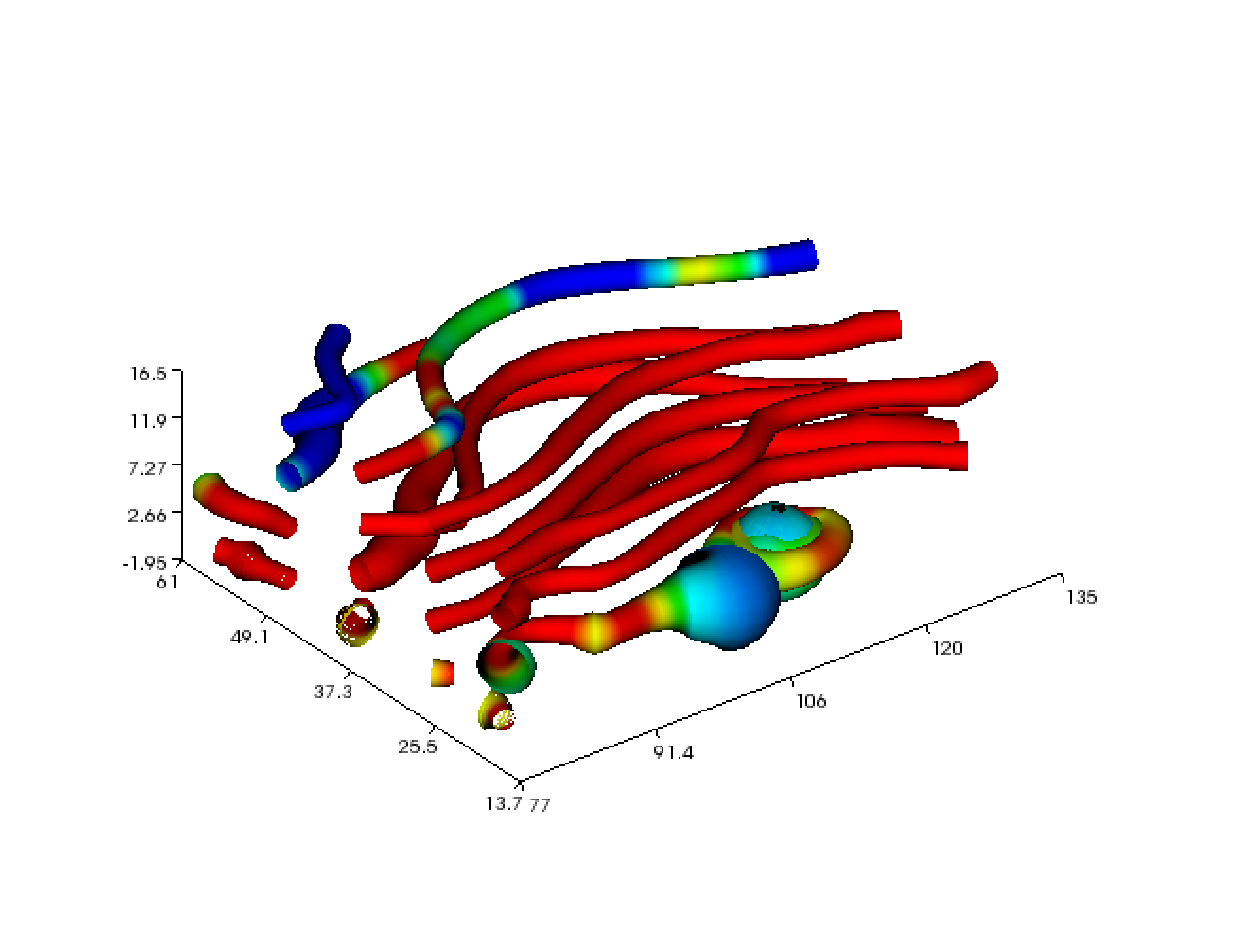
\includegraphics[width=0.9\linewidth]{figs/streamtubes.eps}}
  \caption{
  Streamtube visualization of a fluid flow. \label{fig:viz}
  }
\end{figure}
%\clearpage % flush figures fig:viz


Combining several image files into one, in a table fashion, can be done by the
\Verb!montage! program from the ImageMagick suite:
\begin{Verbatim}[numbers=none,fontsize=\fontsize{9pt}{9pt},baselinestretch=0.95,xleftmargin=0mm]
montage -background white -geometry 100% -tile 2x \
        file1.png file2.png ... file4.png result.png
\end{Verbatim}
The option \Verb!-tile XxY! gives \Verb!X! figures in the horizontal direction and
\Verb!Y! in the vertical direction (\Verb!tile 2x! means two figures per row
and \Verb!-tile x2! means two rows).

\subsection{Movies}

Here is an example on the \Verb!MOVIE:! keyword for embedding movies. This
feature works well for the \Verb!latex!, \Verb!html!, \Verb!rst!, and \Verb!sphinx! formats.
Other formats try to generate some HTML file and link to that file
for showing the movie.
\begin{Verbatim}[numbers=none,fontsize=\fontsize{9pt}{9pt},baselinestretch=0.95,xleftmargin=0mm]
MOVIE: [filename, height=xxx width=yyy] possible caption

\end{Verbatim}

% latex/PDF format can make use of the movie15 package for displaying movies,
% or just plain \href{run: ...}{...}

 (Movie figs/mjolnir.mpeg: play \href{{mjolnir.html}}{\nolinkurl{mjolnir.html}})
\includemedia[
width=0.8\linewidth,
label=figs/mjolnir.mpeg,
activate=pageopen,         % or onclick or pagevisible
addresource=figs/mjolnir.mpeg,  % embed the video in the PDF
flashvars={
source=figs/mjolnir.mpeg
&autoPlay=true
&loop=true
&scaleMode=letterbox   % preserve aspect ration while scaling this video
}]{}{VPlayer.swf}




% MOVIE: [figs/wavepacket.gif, width=600 height=470]

% MOVIE: [figs/wavepacket2.mpeg, width=600 height=470]

The {\LaTeX} format results in a file that can either make use of
the movie15 package (requires the PDF to be shown in Acrobat Reader)
or just a plain address to the movie. The HTML, reST, and
Sphinx formats will play
the movie right away by embedding the file in a standard HTML code,
provided the output format is HTML.
For all other formats a URL to an HTML file, which can play the code,
is inserted in the output document.

When movies are embedded in the PDF file via {\LaTeX} and
the \Verb!movie15! package wanted, one has to turn on the preprocessor
variable \Verb!MOVIE15!. There is an associated variable
\Verb!EXTERNAL_MOVIE_VIEWER! which can be defined to launch an external
viewer when displaying the PDF file (in Acrobat Reader):
\begin{Verbatim}[numbers=none,fontsize=\fontsize{9pt}{9pt},baselinestretch=0.95,xleftmargin=0mm]
Terminal> ptex2tex -DMOVIE15 -DEXTERNAL_MOVIE_VIEWER mydoc
\end{Verbatim}

The HTML, reST, and Sphinx formats can also treat filenames of the form
\Verb!myframes*.png!. In that case, an HTML file for showing the sequence of frames
is generated, and a link to this file is inserted in the output document.
That is, a simple "movie viewer" for the frames is made.

Many publish their scientific movies on YouTube or Vimeo, and Doconce recognizes
YouTube and Vimeo URLs as movies. When the output from Doconce
is an HTML file, the movie will
be embedded, otherwise a URL to the YouTube or Vimeo page is inserted.
You should equip the \Verb!MOVIE:! command with the right width and height
of \emph{embedded} YouTube and Vimeo movies. The recipe goes as follows:

\begin{enumerate}
\item click on \emph{Share} (and on YouTube then \emph{Embed})

\item note the height and width of the embedded movie
\end{enumerate}

\noindent
A typical \Verb!MOVIE! command with a YouTube movie is then

\begin{Verbatim}[numbers=none,fontsize=\fontsize{9pt}{9pt},baselinestretch=0.95,xleftmargin=0mm]
MOVIE: [http://www.youtube.com/watch?v=sI2uCHH3qIM, width=420 height=315]

MOVIE: [http://vimeo.com/55562330, width=500 height=278] CFD.
\end{Verbatim}
Note that there must be a blank line after every \Verb!MOVIE:! command.
The width and height parameters are not required, but leaving them out
may lead to movie sizes you do not want.

 \href{{http://www.youtube.com/watch?v=sI2uCHH3qIM}}{\nolinkurl{http://www.youtube.com/watch?v=sI2uCHH3qIM}}

 CFD. \href{{http://vimeo.com/55562330}}{\nolinkurl{http://vimeo.com/55562330}}

\subsection{Copying Computer Code from Source Files}

Another type of special lines starts with \Verb!@@@CODE! and enables copying
of computer code from a file directly into a verbatim environment, see
Section~\ref{sec:verbatim:blocks} below.


\subsection{Inline Tagging}
\label{inline:tagging}
\index{inline tagging} \index{emphasized words} \index{boldface words} \index{verbatim text}
\index{inline comments}

Doconce supports tags for \emph{emphasized phrases}, \textbf{boldface phrases},
and \Verb!verbatim text! (also called type writer text, for inline code),
\textcolor{blue}{colored words},
plus LaTeX/TeX inline mathematics, such as $\nu = \sin(x)$.

\paragraph{Emphasized Words.}
Emphasized text is typeset inside a pair of asterisk, and there should
be no spaces between an asterisk and the emphasized text, as in
\begin{Verbatim}[numbers=none,fontsize=\fontsize{9pt}{9pt},baselinestretch=0.95,xleftmargin=0mm]
*emphasized words*
\end{Verbatim}

Boldface font is recognized by an underscore instead of an asterisk:
\begin{Verbatim}[numbers=none,fontsize=\fontsize{9pt}{9pt},baselinestretch=0.95,xleftmargin=0mm]
_several words in boldface_ followed by *ephasized text*.
\end{Verbatim}
The line above gets typeset as
\textbf{several words in boldface} followed by \emph{ephasized text}.

\paragraph{Inline Verbatim Text.}
Verbatim text, typically used for short inline code,
is typeset between back-ticks:
\begin{Verbatim}[numbers=none,fontsize=\fontsize{9pt}{9pt},baselinestretch=0.95,xleftmargin=0mm]
`call myroutine(a, b)` looks like a Fortran call
while `void myfunc(double *a, double *b)` must be C.
\end{Verbatim}
The typesetting result looks like this:
\Verb!call myroutine(a, b)! looks like a Fortran call
while \Verb!void myfunc(double *a, double *b)! must be C.

It is recommended to have inline verbatim text on the same line in
the Doconce file, because some formats ({\LaTeX} and \Verb!ptex2tex!) will have
problems with inline verbatim text that is split over two lines.


\begin{graybox1admon}[Notice.]
Watch out for mixing back-ticks and asterisk (i.e., verbatim and
emphasized code): the Doconce interpreter is not very smart so inline
computer code can soon lead to problems in the final format. Go back to the
Doconce source and modify it so the format to which you want to go
becomes correct (sometimes a trial and error process - sticking to
very simple formatting usually avoids such problems).
\end{graybox1admon}

\paragraph{Links to Web Addresses.}
Web addresses with links are typeset as
\begin{Verbatim}[numbers=none,fontsize=\fontsize{9pt}{9pt},baselinestretch=0.95,xleftmargin=0mm]
some URL like "Search Google": "http://google.com".
\end{Verbatim}
which appears as some URL like \href{{http://google.com}}{Search Google}.
The space after colon is optional, but it is important to enclose the
link and the URL in double quotes.

To have the URL address itself as link text, put an "URL" or URL
before the address enclosed in double quotes:
\begin{Verbatim}[numbers=none,fontsize=\fontsize{9pt}{9pt},baselinestretch=0.95,xleftmargin=0mm]
Click on this link: URL:"http://code.google.com/p/doconce".
\end{Verbatim}
which gets rendered as
Click on this link: \href{{http://code.google.com/p/doconce}}{\nolinkurl{http://code.google.com/p/doconce}}.

(There is also support for lazy writing of URLs: any http or https web address
with a leading space and a trailing space, comma, semi-colon, or question
mark (but not period!) becomes a link with the web address as link text.)

\paragraph{Mail Addresses.}
Links that launches a mail to a specified address is written as
ordinary URLs, typically as

\begin{Verbatim}[numbers=none,fontsize=\fontsize{9pt}{9pt},baselinestretch=0.95,xleftmargin=0mm]
Send "mail": "mailto:hpl@simula.no"
# Alternative:
to "`hpl@simula.no`": "mailto:hpl@simula.no".
\end{Verbatim}
which appears as Send \href{{mailto:hpl@simula.no}}{mail} to
\href{{mailto:hpl@simula.no}}{\nolinkurl{hpl@simula.no}}.

\paragraph{Links to Local Files.}
Links to files ending in \Verb!.txt!, \Verb!.html!, \Verb!.pdf!, \Verb!.py!, \Verb!.f!,
\Verb!.f77!, \Verb!.f90!, \Verb!.f95!, \Verb!.sh!, \Verb!.csh!, \Verb!.ksh!, \Verb!.zsh!,
\Verb!.c!, \Verb!.cpp!, \Verb!.cxx!, \Verb!.pl!, and \Verb!.java! follows the same
setup:
\begin{Verbatim}[numbers=none,fontsize=\fontsize{9pt}{9pt},baselinestretch=0.95,xleftmargin=0mm]
see the "Doconce Manual": "manual.do.txt".
\end{Verbatim}
which appears as see the \href{{manual.do.txt}}{Doconce Manual}.
However, linking to local files like this needs caution:

\begin{itemize}
  \item In the \Verb!html! format the links work well if the files are
    supplied with the \Verb!.html! with the same relative location.

  \item In the \Verb!latex! and \Verb!pdflatex! formats, such links in PDF files
    will unless the \Verb!.tex! file has a full URL specified through
    a \Verb!\hyperbaseurl! command and the linked files are located correctly
    relative to this URL. Otherwise full URL must be used in links.

  \item In the \Verb!sphinx! format, links to local files do not work unless the
    files reside in a \Verb!_static! directory (a warning is issued about this).
\end{itemize}

\noindent
As a consequence, we strongly recommend that one copies the relevant
files to a \Verb!_static! or \Verb!_static-name! directory and makes links to
files in this directory only (\Verb!name! is the nickname of the Doconce
document, usually the name of the parent directory or main document).
Other links to files should use the full URL. If Doconce is used
for HTML output only, then plain links to local files work fine.

If you want a link to a local source code file and have it
viewed in the browser rather than being downloaded, we recommend
to transform the source code file to HTML format by running
\Verb!pygmentize!, e.g.,
\begin{Verbatim}[numbers=none,fontsize=\fontsize{9pt}{9pt},baselinestretch=0.95,xleftmargin=0mm]
Terminal> pygmentize -l bash -f html -O full,style=emacs \
          -o _static/make.sh.html subdir/make.sh
\end{Verbatim}
Then you can link to \Verb!_static/make.sh.html! instead of
\Verb!subdir/make.sh!. Here is an example where the reader
has the file available as \Verb!src/myprog.py! in her
software and the document links to \Verb!_static/myprog.py!:
\begin{Verbatim}[numbers=none,fontsize=\fontsize{9pt}{9pt},baselinestretch=0.95,xleftmargin=0mm]
See the code URL:"src/myprog.py" ("view: "_static/myprog.py.html").
\end{Verbatim}

Links to files with other extensions are typeset with
\emph{the filename as link text}. The syntax consists of
the keyword URL, followed by a colon, and then the filename enclosed
in double quotes:
\begin{Verbatim}[numbers=none,fontsize=\fontsize{9pt}{9pt},baselinestretch=0.95,xleftmargin=0mm]
URL: "manual.html"
\end{Verbatim}
resulting in the link \href{{manual.html}}{\nolinkurl{manual.html}}.

% This is now automatically carried out by the autogenerated
% script for sphinx:
% For such local links to
% work with the \Verb!sphinx! format, the \Verb!.rst! file needs a fix, carried
% out by
% !bc sys
% doconce sphinxfix_localURLs mydoc.rst
% !ec
% (The files, such as \Verb!manual.html!, are then copied to a subdirectory
% \Verb!_static!, which must be manually copied to the Sphinx directory's
% \Verb!_static! directory - links in the \Verb!.rst! files are automatically
% adjusted.)

\paragraph{Inline Comments.}
Doconce also supports inline comments in the text:
\begin{Verbatim}[numbers=none,fontsize=\fontsize{9pt}{9pt},baselinestretch=0.95,xleftmargin=0mm]
[name: comment]
\end{Verbatim}
where \Verb!name! is the name of the author of the command, and \Verb!comment! is a
plain text text. Note that there must be a space after the colon,
otherwise the comment is not recognized. \shortinlinecomment{hpl 1}{ Inline comments
can span
several lines,
if desired. }{ Inline comments can span }

The name and comment are visible in the output unless \Verb!doconce format!
is run with a command-line argument \Verb!--skip_inline_comments!
(see Section~\ref{doconce2formats} for an example). Inline comments
are helpful during development of a document since different authors
and readers can comment on formulations, missing points, etc.
All such comments can easily be removed from the \Verb!.do.txt! file
(see Section~\ref{doconce2formats}).

Inline comments are typeset in a simple way (boldface name and the
comment in parenthesis), but in {\LaTeX} very visible color boxes
are used (via the \Verb!todonotes! package).


\paragraph{Inline Mathematics.}
Inline mathematics is written as in {\LaTeX}, i.e., inside dollar signs.
Many formats leave this syntax as it is (including to dollar signs),
hence nice math formatting is only obtained in {\LaTeX}, HTML, MediaWiki,
and Sphinx (Epytext has some inline math support that is utilized).
However, mathematical expressions in {\LaTeX} syntax often contains
special formatting commands, which may appear annoying in plain
text. Doconce therefore supports an extended inline math syntax where
the writer can provide an alternative syntax suited for formats close
to plain ASCII:

\begin{Verbatim}[numbers=none,fontsize=\fontsize{9pt}{9pt},baselinestretch=0.95,xleftmargin=0mm]
Here is an example on a linear system
${\bf A}{\bf x} = {\bf b}$|$Ax=b$,
where $\bf A$|$A$ is an $n\times n$|$nxn$ matrix, and
$\bf x$|$x$ and $\bf b$|$b$ are vectors of length $n$|$n$.
\end{Verbatim}
That is, we provide two alternative expressions, both enclosed in
dollar signs and separated by a pipe symbol, the expression to the
left is used in formats with {\LaTeX} support (\Verb!latex!, \Verb!pdflatex!, \Verb!html!,
\Verb!sphinx!, \Verb!mwiki!), while the expression to the right is used for
all other formats.  The above text is typeset as "Here is an example
on a linear system ${\bf A}{\bf x} = {\bf b}$, where $\bf A$
is an $n\times n$ matrix, and $\bf x$ and $\bf b$
are vectors of length $n$."

\subsection{Comments}

Comments intended to be (sometimes) visible in the output document and
read by readers are known as \emph{inline comments} in Doconce and
described in Section~\ref{inline:tagging}.

Here we address comments in the Doconce source file that are not
intended to be visible in the output document. Basic comment
lines start with the hash \Verb!#!:
\begin{Verbatim}[numbers=none,fontsize=\fontsize{9pt}{9pt},baselinestretch=0.95,xleftmargin=0mm]
#
# Here are some comment lines that do not affect any formatting.
# These lines are converted to comments in the output format.
#
\end{Verbatim}
Such comment lines may have some side effects in the \Verb!rst! and \Verb!sphinx!
formats because following lines are taken as part of the comment if
there is not a blank line after the comment.

The Mako preprocessor supports comments that are filtered out \emph{before}
Doconce starts translating the document. Such comments are very valuable
as they will never interfere with the output format and they are only
present in the Doconce source. Mako has two types of comments:
lines starting with a double hash \Verb!##! and lines enclosed by
the \Verb!<%doc>! (beginning) and \Verb!<%doc/>! (closing) tags.

If you need a lot of comments in the Doconce file, consider using
Mako comments instead of the single hash, unless you want the
comments to be in the source code of the output document.

To comment out or remove large sections, consider using the Preprocess
preprocessor and an if-else block with a variable that is undefined
(typically something like a test \Verb!# #ifdef EXTRA! in Preprocess).


\subsection{Cross-Referencing}
\index{cross referencing} \index{labels} \index{references}

References and labels are supported. The syntax is simple:
\begin{Verbatim}[numbers=none,fontsize=\fontsize{9pt}{9pt},baselinestretch=0.95,xleftmargin=0mm]
label{section:verbatim}   # defines a label
For more information we refer to Section ref{section:verbatim}.
\end{Verbatim}
This syntax is close that that of labels and cross-references in
{\LaTeX}. When the label is placed after a section or subsection heading,
the plain text, Epytext, and StructuredText formats will simply
replace the reference by the title of the (sub)section.  All labels
will become invisible, except those in math environments.  In the
\Verb!rst! and \Verb!sphinx! formats, the end effect is the same, but
the "label" and "ref" commands are first translated to the proper
reST commands by \Verb!doconce format!. In the HTML and (Google
Code) wiki formats, labels become anchors and references become links,
and with {\LaTeX} "label" and "ref" are just equipped with backslashes so
these commands work as usual in {\LaTeX}.

It is, in general, recommended to use labels and references for
(sub)sections, equations, and figures only.
By the way, here is an example on referencing Figure~\ref{fig:viz}
(the label appears in the figure caption in the source code of this document).
Additional references to Sections~\ref{mathtext} and~\ref{newcommands} are
nice to demonstrate, as well as a reference to equations,
say (\ref{myeq1})-(\ref{myeq2}). A comparison of the output and
the source of this document illustrates how labels and references
are handled by the format in question.

Hyperlinks to files or web addresses are handled as explained
in Section~\ref{inline:tagging}.

\subsection{Generalized Cross-Referencing}
\label{manual:genrefs}

Sometimes a series of individual documents may be assembled to one
large document. The assembly impacts how references to sections
are written: when referring to a section in the same document, a label
can be used, while references to sections in other documents are
written differently, sometimes involving a link (URL) and a citation.
Especially if both the individual documents and the large assembly document
are to exist side by side, a flexible way of referencing is needed.
For this purpose, Doconce offers \emph{generalized references} which allows
a reference to have two different formulations, one for internal
references and one for external references. Since {\LaTeX} supports
references to labels in external documents via the \Verb!xr! package,
the generalized references in Doconce has a syntax that may utilize
the \Verb!xr! feature in {\LaTeX}.

The syntax of generalized references reads
\begin{Verbatim}[numbers=none,fontsize=\fontsize{9pt}{9pt},baselinestretch=0.95,xleftmargin=0mm]
ref[internal][cite][external]
\end{Verbatim}
If all \Verb!ref{label}! references in the text \Verb!internal! are references
to labels in the present document, the above \Verb!ref! command is replaced
by the text \Verb!internal!. Otherwise, if cite is non-empty and the format
is \Verb!latex! or \Verb!pdflatex! one assumes that the references in \Verb!internal!
are to external documents declared by a comment line \Verb!# Externaldocuments: testdoc, mydoc! (usually after the title, authors,
and date). In this case the output text is \Verb!internal cite! and the
{\LaTeX} package \Verb!xr! is used to handle the labels in the external documents.
If none of the two situations above applies, the \Verb!external!
text will be the output.

Here is an example on a specific generalized reference:
\begin{Verbatim}[numbers=none,fontsize=\fontsize{9pt}{9pt},baselinestretch=0.95,xleftmargin=0mm]
As explained in
ref[Section ref{subsec:ex}][in "Langtangen, 2012":
"http://code.google.com/p/doconce/wiki/Description"
cite{testdoc:12}][a "section": "testdoc.html#___sec2" in
the document "A Document for Testing Doconce": "testdoc.html"
cite{testdoc:12}], Doconce documents may include movies.
\end{Verbatim}
In {\LaTeX}, this becomes
\begin{Verbatim}[numbers=none,fontsize=\fontsize{9pt}{9pt},baselinestretch=0.95,xleftmargin=0mm]
As explained in
Section~\ref{subsec:ex} in
\href{{http://code.google.com/p/doconce/source/browse/test/testdoc.do.txt}}{Langtangen, 2012}
\cite{testdoc:12}, Doconce documents may include movies.
\end{Verbatim}
Note that there is a specific numbered reference to an external
document, if \Verb!subsec:ex! is not a label in the present document,
and that we add a citation in the usual way, but also include
a link to the document using the name of the other or some other
relevant link text. The link can be the same or different from
links used in the "external" part of the reference ({\LaTeX} cannot
have links to local files, so a complete URL must be used).

Translation to Sphinx or reStructuredText results in
\begin{Verbatim}[numbers=none,fontsize=\fontsize{9pt}{9pt},baselinestretch=0.95,xleftmargin=0mm]
As explained in
a `section <testdoc.html#___sec2>`_ in
the document `A Document for Testing Doconce <testdoc.html>`_
[testdoc:12]_, Doconce documents may include movies.
\end{Verbatim}
In plain HTML, this becomes
\begin{Verbatim}[numbers=none,fontsize=\fontsize{9pt}{9pt},baselinestretch=0.95,xleftmargin=0mm]
As explained in
a <a href="testdoc.html#___sec2">section</a> in
the document <a href="testdoc.html">A Document for Testing Doconce</a>
<a href="#testdoc:12">[1]</a>, Doconce documents may include movies.
\end{Verbatim}
The plain text format reads
\begin{Verbatim}[numbers=none,fontsize=\fontsize{9pt}{9pt},baselinestretch=0.95,xleftmargin=0mm]
As explained in
a section (testdoc.html#___sec2) in
the document A Document for Testing Doconce (testdoc.html)
[1], Doconce documents may include movies.
\end{Verbatim}
And in Pandoc-exteded Markdown we have
\begin{Verbatim}[numbers=none,fontsize=\fontsize{9pt}{9pt},baselinestretch=0.95,xleftmargin=0mm]
As explained in
a [section](testdoc.html#___sec2) in
the document [A Document for Testing Doconce](testdoc.html)
@testdoc:12, Doconce documents may include movies.
\end{Verbatim}

\subsection{Index}
\index{index} \index{citations} \index{bibliography}

An index can be created for the \Verb!latex!, \Verb!rst!, and \Verb!sphinx! formats
by the \Verb!idx! keyword, following a LaTeX-inspired syntax:
\begin{Verbatim}[numbers=none,fontsize=\fontsize{9pt}{9pt},baselinestretch=0.95,xleftmargin=0mm]
idx{some index entry}
idx{main entry!subentry}
idx{`verbatim_text` and more}
\end{Verbatim}
The exclamation mark divides a main entry and a subentry. Backquotes
surround verbatim text, which is correctly transformed in a {\LaTeX} setting to
\begin{Verbatim}[numbers=none,fontsize=\fontsize{9pt}{9pt},baselinestretch=0.95,xleftmargin=0mm]
\index{verbatim\_text@\texttt{\rm\smaller verbatim\_text and more}}
\end{Verbatim}
Everything related to the index simply becomes invisible in plain
text, Epytext, StructuredText, HTML, and wiki formats.  Note: \Verb!idx!
commands should be inserted outside paragraphs, not in between the
text as this may cause some strange behaviour of reST and
Sphinx formatting.  As a recommended rule, index items are naturally
placed right after section headings, before the text begins, while
index items related to a paragraph should be placed above the
paragraph one a separate line (and not in between the text or between
the paragraph heading and the text body, although this works fine if
{\LaTeX} is the output format). For paragraphs with \Verb!===! heading,
the index keywords should be placed above the heading.

The keywords in the index are automatically placed in a meta
tag in \Verb!html! output such that search engines can make use of the them.

\subsection{Bibliography}

Doconce applies the software tool \href{{https://bitbucket.org/logg/publish}}{Publish} to handle the bibliography in a
document. With Publish it is easy to import \textsc{Bib}\negthinspace{\TeX} data and maintain a
database in a clean, self-explanatory textual format. From the Publish
format it is easy to go \textsc{Bib}\negthinspace{\TeX} and reST or straightforward Doconce
typesetting (and from there to HTML, plain text, wiki formats, and so
on).

Installing Publish is straightforward: just checkout the code on
\href{{https://bitbucket.org/logg/publish}}{\nolinkurl{bitbucket.org}}, move to the
\Verb!publish! directory and run \Verb!sudo python setup.py install!.

\paragraph{Importing your data to the Publish database.}
Many scientists have their bibliographic data in the BibTex format. Here we
assume that you have two files, \Verb!refs1.bib! and \Verb!refs2.bib!. These can
be imported to a Publish database, residing in the file \Verb!papers.pub!,
by the commands

\begin{Verbatim}[numbers=none,fontsize=\fontsize{9pt}{9pt},baselinestretch=0.95,xleftmargin=0mm]
publish import refs1.bib
publish import refs2.bib
\end{Verbatim}
During import, Publish may ask you for accepting the name of new
institutions or journals. Publish already have a database of journals
and institutions/departments, but when you add new, you also get
a file \Verb!venues.list! (in the current working directory) which will be used
for future imports in this directory. Make sure you store \Verb!publish.pub!
and \Verb!venues.list! along with your Doconce document files (e.g., add them to
your version control system).

\paragraph{Requirements to input data.}

\begin{graybox1admon}[Notice.]
Note that Publish only accepts \textsc{Bib}\negthinspace{\TeX} files where the keys (author,
title, etc.) are in lower case and where the data are enclosed in
curly braces. You may need to edit your \textsc{Bib}\negthinspace{\TeX} files to meet this
demand.
\end{graybox1admon}

The utility \Verb!doconce fix_bibtex4publish file.bib! fixes several known
issues with \textsc{Bib}\negthinspace{\TeX} files such that Publish has a better chance of
accepting the entries. Run this utility first, then run Publish,
respond to any requirements that Publish spits out, remove \Verb!papers.pub!
if it exists, and run the import statements again.

Although references are visible as numbers only in the
output, it is recommended to have apply a nice, consistent
typesetting of your keys. It is suggested to use the following scheme:

\begin{Verbatim}[numbers=none,fontsize=\fontsize{9pt}{9pt},baselinestretch=0.95,xleftmargin=0mm]
Langtangen_2003a          # single author
Langtangen_Pedersen_2002  # two authors
Langtangen_et_al_2002     # three or more authors
\end{Verbatim}
One can add a, b, c, and so forth if several keys feature the same
authors and year.

\paragraph{Adding new references to the database.}
When you get some new \textsc{Bib}\negthinspace{\TeX} references you simply put them in
a file, say \Verb!refs3.pub! and run the \Verb!publish import refs3.pub! command
to update the database. You may also consider editing the \Verb!papers.pub!
file directly when adding new references.

\paragraph{Exporting the database.}
Export of everything in the database to
\textsc{Bib}\negthinspace{\TeX} is done by

\begin{Verbatim}[numbers=none,fontsize=\fontsize{9pt}{9pt},baselinestretch=0.95,xleftmargin=0mm]
publish export mybibtexfile.bib
\end{Verbatim}
You can easily export subsets of the database, e.g., only papers associated
with a particular author (the Publish manual has details on how this is
done). Doconce will automatically export the database to \textsc{Bib}\negthinspace{\TeX} if
the output format is \Verb!latex! or \Verb!pdflatex!.

\paragraph{Referring to publications.}
We use the command

\begin{Verbatim}[numbers=none,fontsize=\fontsize{9pt}{9pt},baselinestretch=0.95,xleftmargin=0mm]
cite{key}
\end{Verbatim}
to refer to a publication with bibliographic key \Verb!key!.
Here is an example: \cite{Langtangen_Pedersen_2002} discussed propagation of
large destructive water waves, \cite{Langtangen_et_al_2002} gave
an overview of numerical methods for solvin the Navier-Stokes equations,
while the use of Backward Kolmogorov equations for analyzing
random vibrations was investigated in \cite{Langtangen_1994a}.
The book chapter \cite{Mardal_et_al_2003a} contains information on
C++ software tools for programming multigrid methods. A real retro
reference is \cite{Langtangen_1988d} about a big FORTRAN package.
Multiple references are also possible, e.g., see
\cite{Langtangen_Pedersen_2002,Mardal_et_al_2003a}.

In {\LaTeX}, the \Verb!cite! command is directly translated to the
corresponding {\LaTeX} version of the command with a backslash; in reST
and Sphinx the citations becomes links, with the citation keys as
names; in HTML the citations are numbered from 1, 2, and so forth
according to their appearance, and the numbers appear as links; while
in other formats the citations are simply the keys inside square
brackets and the corresponding references are listed in the order they
are cited.

\paragraph{Specifying the Publish database.}
The specification of the Publish database file in the Doconce document
is done one a line containing \Verb!BIBFILE: papers.pub! (you may give
the database file another name and store it in another directory).
The references will be inserted at the place where this command appears.
Before the command you will often want to have a headline with
"References", "Bibliography", or similar.
Here is an example:

\begin{Verbatim}[numbers=none,fontsize=\fontsize{9pt}{9pt},baselinestretch=0.95,xleftmargin=0mm]

======= References =======

BIBFILE: papers.pub
\end{Verbatim}
In {\LaTeX} and \textsc{pdf}{\LaTeX} the \Verb!papers.pub! file is exported to \textsc{Bib}\negthinspace{\TeX} format
and included in the document, while in all other formats, suitable
text is produced from the database.

\paragraph{{\LaTeX} bibliography style.}
The bibliography style is "plain" in {\LaTeX} output. To change this, just
edit the \Verb!.p.tex! file. For example,

\begin{Verbatim}[numbers=none,fontsize=\fontsize{9pt}{9pt},baselinestretch=0.95,xleftmargin=0mm]
doconce format latex mydoc
doconce replace 'bibliographystyle{plain}' 'bibliographystyle{abbrev}' mydoc.p.tex
\end{Verbatim}

\subsection{Tables}

A table like


\begin{quote}\begin{tabular}{rrr}
\hline
\multicolumn{1}{c}{ time } & \multicolumn{1}{c}{ velocity } & \multicolumn{1}{c}{ acceleration } \\
\hline
0.0          & 1.4186       & -5.01        \\
2.0          & 1.376512     & 11.919       \\
4.0          & 1.1E+1       & 14.717624    \\
\hline
\end{tabular}\end{quote}

\noindent
is built up of pipe symbols and dashes:
\begin{Verbatim}[numbers=none,fontsize=\fontsize{9pt}{9pt},baselinestretch=0.95,xleftmargin=0mm]
  |--------------------------------|
  |time  | velocity | acceleration |
  |--------------------------------|
  | 0.0  | 1.4186   | -5.01        |
  | 2.0  | 1.376512 | 11.919       |
  | 4.0  | 1.1E+1   | 14.717624    |
  |--------------------------------|
\end{Verbatim}
The pipes and column values do not need to be aligned (but why write
the Doconce source in an ugly way?). In the line below the heading,
one can insert the characters \Verb!c!, \Verb!r!, or \Verb!l! to specify the
alignment of the columns (centered, right, or left, respectively).
Similar character can be inserted in the line above the header to
algn the headings. Pipes \Verb!|! can also be inserted to indicate
vertical rules in {\LaTeX} tables (they are ignored for other formats).
An example of centered headings (which is default anyway), first
column left-adjusted and the others right-adjusted looks like

\begin{Verbatim}[numbers=none,fontsize=\fontsize{9pt}{9pt},baselinestretch=0.95,xleftmargin=0mm]
  |--c--------c-----------c--------|
  |time  | velocity | acceleration |
  |--l--------r-----------r--------|
  | 0.0  | 1.4186   | -5.01        |
  | 2.0  | 1.376512 | 11.919       |
  | 4.0  | 1.1E+1   | 14.717624    |
  |--------------------------------|
\end{Verbatim}

Note that not all formats offer alignment of heading or entries
in tables (\Verb!rst! and \Verb!sphinx! are examples). Also note that
Doconce tables are very simple: neither entries nor
headings can span several columns or rows. When that functionality
is needed, one can make use of the preprocessor and if-tests on
the format and insert format-specific code for tables.

The command-line option \Verb!--tables2csv! (to \Verb!doconce format!)
makes Doconce dump each table to CSV format in a file \Verb!table_X.csv!,
where \Verb!X! is the table number. This feature makes it easy to
load tables into spreadsheet programs for further analysis.

Data in CSV format can be transformed to Doconce table format
by the \Verb!doconce csv2table! utility:

\begin{Verbatim}[numbers=none,fontsize=\fontsize{9pt}{9pt},baselinestretch=0.95,xleftmargin=0mm]
Terminal> doconce csv2table somefile.csv > table.do.txt
\end{Verbatim}
This is a quick way of writing tables. For example, we can
write a text file \Verb!tmp.csv! with

\begin{Verbatim}[numbers=none,fontsize=\fontsize{9pt}{9pt},baselinestretch=0.95,xleftmargin=0mm]
time, velocity, acceleration
0.0, 1.4186, -5.01
2.0, 1.376512, 11.919
4.0, 1.1E+1, 14.717624
\end{Verbatim}
Running \Verb!doconce csv2table tmp.csv! creates the table

\begin{Verbatim}[numbers=none,fontsize=\fontsize{9pt}{9pt},baselinestretch=0.95,xleftmargin=0mm]
|------c--------------c--------------c-------|
| time         | velocity     | acceleration |
|------c--------------c--------------c-------|
| 0.0          | 1.4186       | -5.01        |
| 2.0          | 1.376512     | 11.919       |
| 4.0          | 1.1E+1       | 14.717624    |
|--------------------------------------------|
\end{Verbatim}

\subsection{Exercises, Problems, Projects, and Examples}

Doconce has special support for four types of "exercises", named
\emph{exercise}, \emph{problem}, \emph{project}, or \emph{example}.
These are all typeset as special kind of
sections. Such sections start with a subsection
headline, 5 \Verb!=! characters, and last up to the
next headline or the end of the file. The headline itself must
consists of the word "Exercise", "Problem", "Project", or "Example", followed
by a colon and a title of the exercise, problem, or project.
The next line(s) may contain a label and specification of the
name of result file (if the answer to the exercise is to be handed
in) and a solution file. The Doconce code looks like this:

\begin{Verbatim}[numbers=none,fontsize=\fontsize{9pt}{9pt},baselinestretch=0.95,xleftmargin=0mm]
===== Project: Determine the Distance to the Moon =====
label{proj:moondist}
file=earth2moon.pdf
solution=eart2moon_sol.do.txt

Here goes the running text of the project....

\end{Verbatim}
Doconce will recognize the exercise, problem, project, or example \emph{title},
the \emph{label}, the \emph{result file}, the \emph{solution} (if any of
these three entities is present), and the \emph{running text}. In addition,
one can add subexercise environments, starting with \Verb!!bsubex! and ending
with \Verb!!esubex!, on the beginning of separate lines.
Within the main exercise or
a subexercise, three other environments are possible: (full) solution,
(short) \emph{answer}, and \emph{hints}. The environments have begin-end
directives \Verb!!bans!, \Verb!!eans!, \Verb!!bsol!, \Verb!!esol!, \Verb!!bhint!, \Verb!!ehint!, which
all must appear on the beginning of a separate line (just as
\Verb!!bc! and \Verb!!ec!).

The solution environment allows inline
solution as an alternative to the \Verb!solution=...! directive mentioned above,
which requires that the solution is in a separate file. Comment lines
are inserted so that the beginning and end of answers and solutions can
be identified and removed if desired.

A full exercise set-up can be sketched as follows:
\begin{Verbatim}[numbers=none,fontsize=\fontsize{9pt}{9pt},baselinestretch=0.95,xleftmargin=0mm]
===== Exercise: Determine the Distance to the Moon =====
label{exer:moondist}
file=earth2moon.pdf

Here goes main body of text describing the exercise...

!bsubex
Subexercises are numbered a), b), etc.

!bans
Short answer to subexercise a).
!eans

!bhint
First hint to subexercise a).
!ehint

!bhint
Second hint to subexercise a).
!ehint
!esubex

!bsubex
Here goes the text for subexercise b).

!bhint
A hint for this subexercise.
!ehint

!bsol
Here goes the solution of this subexercise.
!esol
!esubex

!bremarks
At the very end of the exercise it may be appropriate to summarize
and give some perspectives. The text inside the !bremarks-!eremarks
directives is always typeset at the end of the exercise.
!eremarks

!bsol
Here goes a full solution of the whole exercise.
!esol
!ec

A recommended rule for using the different "exercise" types goes as follows:

  * Exercises are smaller problems directly related to the present chapter
    (e.g., with references to the text).
  * Problems are sufficiently independent of the chapter's text
    that they make sense on their own, separated from the rest of the docoment.
  * Projects are larger problems that also make sense on their own.
  * Examples are exercises, problems, or projects with full solutions.

The command line options `--without_answers` and `--without_solutions`
turn off output of answers and solutions, respectively, except for
examples.

Sometimes one does not want the heading of an exercise, problem, project,
or example to contain the keyword `Exercise:`, `Problem:`, `Project:`,
or `Example:`. By enclosing the keyword in braces, as in

\begin{Verbatim}[numbers=none,fontsize=\fontsize{9pt}{9pt},baselinestretch=0.95,xleftmargin=0mm]
===== {Problem}: Find a solution to a problem =====
\end{Verbatim}
the keyword is marked for being left out of the heading, resulting in
the heading "Find a solution to a problem".


The various elements of exercises are collected in a special data
structure (list of dictionaries) stored in a file \Verb!.mydoc.exerinfo!,
if \Verb!mydoc.do.txt! is the name of the Doconce file.  The file contains
a list of dictionaries, where keys in the dictionary corresponds to
elements in the exercise: filename, solution file, answer, label, list
of hints, list of subexercises, closing remarks, and the main body of
text. From this data structure it is easy to generate stand-alone
documents with exercises, problems, and projects with or without
short answers and full solutions.

Tailored formatting of exercises in special output formats can make
use of the elements in an exercise.  For example, one can image web
formats where the hints are displayed one by one when needed and where
the result file can be uploaded. One can also think of mechanisms for
downloading the solution file if the result file meets certain
criteria.  Doconce does not yet generate such functionality in any
output format, but this is an intended future feature to be
impelemented.

For now, exercises, problems, projects, examples are typeset as ordinary
Doconce sections (this is the most general approach that will work for many
formats). One must therefore refer to an exercise, problem, project, or
example by its label, which normally will translate to the section number
(in {\LaTeX}, for instance) or a link to the title of the section.
The \emph{title} is typeset without any leading "Exercise:", "Problem:",
or "Project:" word, so that references like
\begin{Verbatim}[numbers=none,fontsize=\fontsize{9pt}{9pt},baselinestretch=0.95,xleftmargin=0mm]
see Problem ref{...}
\end{Verbatim}
works well in all formats (i.e., no double "Problem Problem" appears).

\paragraph{Remark.}
Examples are \emph{not} typeset similarly to exercises unless one adds
the command-line option \Verb!--examples_as_exercises!. That is, without
this option, any heading and starting with \Verb!Example:! makes Doconce
treat the forthcoming text as ordinary text without any interpretation
of exercise-style instructions.
With the command-line option \Verb!--examples_as_exercises!,
one can use the \Verb!!bsubex! and \Verb!!bsol!
commands to indicate a subproblem and a solution. In this way, the
typesetting of the example looks like an exercise equipped with a solution.



\subsection{Blocks of Verbatim Computer Code}
\label{sec:verbatim:blocks}

Blocks of computer code, to be typeset verbatim, must appear inside a
"begin code" \Verb!!bc! keyword and an "end code" \Verb!!ec! keyword. Both
keywords must be on a single line and \emph{start at the beginning of the
line}.  Before such a code block there must be a plain sentence
(at least if successful transformation to reST and
ASCII-type formats is desired). For example, a code block cannot come
directly after a section/paragraph heading or a table.

Here is a plain code block:

\begin{Verbatim}[numbers=none,fontsize=\fontsize{9pt}{9pt},baselinestretch=0.95,xleftmargin=0mm]
!bc
% Could be a comment line in some file
% And some data
1.003 1.025
2.204 1.730
3.001 1.198
!ec
\end{Verbatim}
which gets rendered as

\begin{Verbatim}[numbers=none,fontsize=\fontsize{9pt}{9pt},baselinestretch=0.95,xleftmargin=0mm]
% Could be a comment line in some file
% And some data
1.003 1.025
2.204 1.730
3.001 1.198
\end{Verbatim}


There may be an argument after the \Verb!!bc! tag to specify a certain
environment (for \Verb!ptex2tex!, \Verb!doconce ptex2tex!, or Sphinx) for
typesetting the verbatim code. For instance, \Verb!!bc dat! corresponds to
the data file environment and \Verb!!bc cod! is typically used for a code
snippet. There are some predefined environments explained below. If
there is no argument specifying the environment, one assumes some
plain verbatim typesetting (for \Verb!ptex2tex! this means the \Verb!ccq!
environment, which is defined in the config file \Verb!.ptex2tex.cfg!,
while for Sphinx it defaults to the \Verb!python! environment).

Since the config file for \Verb!ptex2tex! and command-line arguments for
the alternative \Verb!doconce ptex2tex! program can define what some environments
map onto with respect to typesetting, a similar possibility is
supported for Sphinx as well.  The argument after \Verb!!bc! is in case of
Sphinx output mapped onto a valid Pygments language for typesetting of
the verbatim block by Pygments. This mapping takes place in an
optional comment to be inserted in the Doconce source file, e.g.,
\begin{Verbatim}[numbers=none,fontsize=\fontsize{9pt}{9pt},baselinestretch=0.95,xleftmargin=0mm]
# sphinx code-blocks: pycod=python cod=fortran cppcod=c++ sys=console
\end{Verbatim}
Here, three arguments are defined: \Verb!pycod! for Python code,
\Verb!cod! also for Python code, \Verb!cppcod! for C++ code, and \Verb!sys!
for terminal sessions. The same arguments would be defined
in \Verb!.ptex2tex.cfg! for how to typeset the blocks in {\LaTeX} using
various verbatim styles (Pygments can also be used in a {\LaTeX}
context).

By default, \Verb!pro! is used for complete programs in Python, \Verb!cod! is
for a code snippet in Python, while \Verb!xcod! and \Verb!xpro! implies computer
language specific typesetting where \Verb!x! can be \Verb!f! for Fortran, \Verb!c!
for C, \Verb!cpp! for C++, \Verb!sh! for Unix shells, \Verb!pl! for Perl, \Verb!m! for
Matlab, \Verb!cy! for Cython, and \Verb!py! for Python.  The argument \Verb!sys!
means by default \Verb!console! for Sphinx and \Verb!CodeTerminal! (ptex2tex
environent) for {\LaTeX}. Other specifications are \Verb!dat! for a data file
or print out, and \Verb!ipy! for interactive Python sessions (the latter
does not introduce any environment  in \Verb!sphinx! output, as interactive
sessions are automatically recognized and handled).  All these
definitions of the arguments after \Verb!!bc! can be redefined in the
\Verb!.ptex2tex.cfg! configuration file for ptex2tex/LaTeX and in the
\Verb!sphinx code-blocks! comments for Sphinx. Support for other languages
is easily added.

% (Any sphinx code-block comment, whether inside verbatim code
% blocks or outside, yields a mapping between bc arguments
% and computer languages. In case of muliple definitions, the
% first one is used.)

The enclosing \Verb!!ec! tag of verbatim computer code blocks must
be followed by a newline.  A common error in list environments is to
forget to indent the plain text surrounding the code blocks. In
general, we recommend to use paragraph headings instead of list items
in combination with code blocks (it usually looks better, and some
common errors are naturally avoided).

Here is a verbatim code block with Python code (\Verb!pycod! style):
\begin{Verbatim}[numbers=none,fontsize=\fontsize{9pt}{9pt},baselinestretch=0.95,xleftmargin=0mm]
!bc pycod
# regular expressions for inline tags:
inline_tag_begin = r'(?P<begin>(^|\s+))'
inline_tag_end = r'(?P<end>[.,?!;:)\s])'
INLINE_TAGS = {
    'emphasize':
    r'%s\*(?P<subst>[^ `][^*`]*)\*%s' % \
    (inline_tag_begin, inline_tag_end),
    'verbatim':
    r'%s`(?P<subst>[^ ][^`]*)`%s' % \
    (inline_tag_begin, inline_tag_end),
    'bold':
    r'%s_(?P<subst>[^ `][^_`]*)_%s' % \
    (inline_tag_begin, inline_tag_end),
}
!ec
\end{Verbatim}
The typeset result of this block becomes

\begin{Verbatim}[numbers=none,fontsize=\fontsize{9pt}{9pt},baselinestretch=0.95,xleftmargin=0mm]
# regular expressions for inline tags:
inline_tag_begin = r'(?P<begin>(^|\s+))'
inline_tag_end = r'(?P<end>[.,?!;:)\s])'
INLINE_TAGS = {
    'emphasize':
    r'%s\*(?P<subst>[^ `][^*`]*)\*%s' % \
    (inline_tag_begin, inline_tag_end),
    'verbatim':
    r'%s`(?P<subst>[^ ][^`]*)`%s' % \
    (inline_tag_begin, inline_tag_end),
    'bold':
    r'%s_(?P<subst>[^ `][^_`]*)_%s' % \
    (inline_tag_begin, inline_tag_end),
}
\end{Verbatim}
And here is a C++ code snippet (\Verb!cppcod! style):
\begin{Verbatim}[numbers=none,fontsize=\fontsize{9pt}{9pt},baselinestretch=0.95,xleftmargin=0mm]
void myfunc(double* x, const double& myarr) {
    for (int i = 1; i < myarr.size(); i++) {
        myarr[i] = myarr[i] - x[i]*myarr[i-1]
    }
}
\end{Verbatim}

% When showing copy from file in !bc envir, intent a character - otherwise
% ptex2tex is confused and starts copying. However, here (in make.sh) we use
% doconce ptex2tex which does not have this problem.
Computer code can be copied directly from a file, if desired. The syntax
is then
\begin{Verbatim}[numbers=none,fontsize=\fontsize{9pt}{9pt},baselinestretch=0.95,xleftmargin=0mm]
@@@CODE myfile.f
@@@CODE myfile.f fromto: subroutine\s+test@^C\s{5}END1
\end{Verbatim}
The first line implies that all lines in the file \Verb!myfile.f! are
copied into a verbatim block, typset in a \Verb!!bc Xpro! environment, where
\Verb!X! is the extension of the filename, here \Verb!f! (i.e., the environment
becomes \Verb!!bc fpro! and will typically lead to some Fortran-style
formatting in Linux and Sphinx).  The
second line has a \Verb!fromto:! directive, which implies copying code
between two lines in the code, typset within a !`bc Xcod`
environment (again, \Verb!X! is the filename extension, implying the
type of file). Note that the \Verb!pro! and \Verb!cod! arguments are only used for {\LaTeX}
and Sphinx output, all other formats will have the code typeset within
a plain \Verb!!bc! environment.) Two regular expressions, separated by the
\Verb!@! sign, define the "from" and "to" lines.  The "from" line is
included in the verbatim block, while the "to" line is not. In the
example above, we copy code from the line matching \Verb!subroutine test!
(with as many blanks as desired between the two words) and the line
matching \Verb!C END1! (C followed by 5 blanks and then the text END1). The
final line with the "to" text is not included in the verbatim block.

Let us copy a whole file (the first line above):

\begin{Verbatim}[numbers=none,fontsize=\fontsize{9pt}{9pt},baselinestretch=0.95,xleftmargin=0mm]
C     a comment

      subroutine test()
      integer i
      real*8 r
      r = 0
      do i = 1, i
         r = r + i
      end do
      return
C     END1

      program testme
      call test()
      return
\end{Verbatim}

Let us then copy just a piece in the middle as indicated by the \Verb!fromto:!
directive above:

\begin{Verbatim}[numbers=none,fontsize=\fontsize{9pt}{9pt},baselinestretch=0.95,xleftmargin=0mm]
      subroutine test()
      integer i
      real*8 r
      r = 0
      do i = 1, i
         r = r + i
      end do
      return
\end{Verbatim}

Note that the "to" line is not copied into the Doconce file, but the
"from" line is. Sometimes it is convenient to also neglect the
"from" line, a feature that is allowed by replacing \Verb!fromto:! by
\Verb!from-to! ("from with minus"). This allows for copying very similar
code segments throughout a file, while still distinguishing between them.
Copying the second set of parameters from the text
\begin{Verbatim}[numbers=none,fontsize=\fontsize{9pt}{9pt},baselinestretch=0.95,xleftmargin=0mm]
# --- Start Example 1 ---
c = -1
A = 2
p0 = 4
simulate_and_plot(c, A, p0)
# --- End Example 1 ---

# --- Start Example 2 ---
c = -1
A = 1
p0 = 0
simulate_and_plot(c, A, p0)
# --- End Example 2 ---
\end{Verbatim}
is easy with
\begin{Verbatim}[numbers=none,fontsize=\fontsize{9pt}{9pt},baselinestretch=0.95,xleftmargin=0mm]
from-to: Start Example 2@End Example 2
\end{Verbatim}
With only \Verb!fromto:! this would be impossible.

(Remark for those familiar with \Verb!ptex2tex!: The from-to
syntax is slightly different from that used in \Verb!ptex2tex!. When
transforming Doconce to {\LaTeX}, one first transforms the document to a
\Verb!.p.tex! file to be treated by \Verb!ptex2tex!. However, the \Verb!@@@CODE! line
is interpreted by Doconce and replaced by the mentioned
pro or cod environment which are defined in the \Verb!ptex2tex! configuration
file.)


\subsection{{\LaTeX} Blocks of Mathematical Text}
\label{mathtext}

Blocks of mathematical text are like computer code blocks, but
the opening tag is \Verb!!bt! (begin TeX) and the closing tag is
\Verb!!et!. It is important that \Verb!!bt! and \Verb!!et! appear on the beginning of the
line and followed by a newline.
\begin{Verbatim}[numbers=none,fontsize=\fontsize{9pt}{9pt},baselinestretch=0.95,xleftmargin=0mm]
!bt
\begin{align}
{\partial u\over\partial t} &= \nabla^2 u + f, label{myeq1}\\
{\partial v\over\partial t} &= \nabla\cdot(q(u)\nabla v) + g. label{myeq2}
\end{align}
!et
\end{Verbatim}

The support of {\LaTeX} mathematics varies among the formats:

\begin{itemize}
 \item Output in {\LaTeX} (\Verb!latex! and \Verb!pdflatex! formats) has of course full
   support of all {\LaTeX} mathematics, of course.

 \item The \Verb!html! format supports single equations and multiple equations
   via the align environment, also with labels.

 \item Markdown (\Verb!pandoc! format) allows single equations and inline mathematics.

 \item MediaWiki (\Verb!mwiki! format) does not enable labels in equations and hence
   equations cannot be referred to.
\end{itemize}

\noindent
The main conclusion is that for
output beyond {\LaTeX} (\Verb!latex! and \Verb!pdflatex! formats), stick to
simple \Verb!\[! and \Verb!\]! or \Verb!equation! and \Verb!align! or \Verb!align*! environments,
and avoid referring to equations in MediaWikis.

Going from Doconce to MS Word is most easily done by outputting in
the \Verb!latex! format and then using the Pandoc program to translate
from {\LaTeX} to MS Word (note that only a subset of {\LaTeX} will be
translated correctly).

If the document targets formats with and without support of {\LaTeX}
mathematics, one can use the preprocessor to typeset the mathematics
in two versions. After \Verb!#if FORMAT in ("latex", "pdflatex", "html", "sphinx", "mwiki", "pandoc")! one places {\LaTeX} mathematics, and after
\Verb!#else! one can write inline mathematics in a way that looks nice in
plain text and wiki formats without support for mathematical
typesetting. Such branching can be used with mako if-else statements
alternatively:

\begin{Verbatim}[numbers=none,fontsize=\fontsize{9pt}{9pt},baselinestretch=0.95,xleftmargin=0mm]
% if FORMAT in ("latex", "pdflatex", "html", "sphinx", "mwiki", "pandoc"):
!bt
\[ \sin^2x + \cos^2x = 1,\]
!et
% else:
!bc
              sin^2(x) + cos^2(x) = 1,
!ec
% endif
\end{Verbatim}


\paragraph{Mathematics for PowerPoint/OpenOffice.}
If you have {\LaTeX} mathematics written in Doconce, it is fairly easy
to generate PNG images of all mathematical formulas and equations for
use with PowerPoint or OpenOffice presentations.

\begin{enumerate}
 \item Make a Sphinx version of the Doconce file.

 \item Go to the Sphinx directory and load the \Verb!conf.py! file into
    a browser.

 \item Search for "math" and comment out the
    \Verb!'sphinx.ext.mathjax'! (enabled by default) and
    \Verb!'matplotlib.sphinxext.mathmpl'! (disabled by default)
    lines, and uncomment the \Verb!'sphinx.ext.pngmath'! package.
    This is the package that generates small PNG pictures
    of the mathematics.

 \item Uncomment the line with \Verb!pngmath_dvipng_args =! and
    set the PNG resolution to \Verb!-D 200! when the purpose is to
    generate mathematics pictures for slides.

 \item Run \Verb!make html!.

 \item Look at the HTML source file in the \Verb!_build/html!
    directory: all mathematics are in \Verb!img! tags with \Verb!src=!
    pointing to a PNG file and \Verb!alt=! pointing to the {\LaTeX}
    source for the formula in question. This makes it very
    easy to find the PNG file that corresponding to a particular
    mathematical expression.
\end{enumerate}

\noindent
\subsection{Macros (Newcommands)}
\label{newcommands}

Doconce supports a type of macros via a LaTeX-style \emph{newcommand}
construction.  The newcommands defined in a file with name
\Verb!newcommand_replace.tex! are expanded when Doconce is filtered to
other formats, except for {\LaTeX} (since {\LaTeX} performs the expansion
itself).  Newcommands in files with names \Verb!newcommands.tex! and
\Verb!newcommands_keep.tex! are kept unaltered when Doconce text is
filtered to other formats, except for the Sphinx format. Since Sphinx
understands {\LaTeX} math, but not newcommands if the Sphinx output is
HTML, it makes most sense to expand all newcommands.  Normally, a user
will put all newcommands that appear in math blocks surrounded by
\Verb!!bt! and \Verb!!et! in \Verb!newcommands_keep.tex! to keep them unchanged, at
least if they contribute to make the raw {\LaTeX} math text easier to
read in the formats that cannot render {\LaTeX}.  Newcommands used
elsewhere throughout the text will usually be placed in
\Verb!newcommands_replace.tex! and expanded by Doconce.  The definitions of
newcommands in the \Verb!newcommands*.tex! files \emph{must} appear on a single
line (multi-line newcommands are too hard to parse with regular
expressions).


\subsection{Admonitions}

Doconce offers strong support for admonition environments, such
as warning boxes, notification boxes, question boxes,
and summary boxes. The boxes normally have an icon, a heading,
and may also have a background color. A special box, the block,
has never any icon and can be used when an icon would be disturbing
or misleading.

The following admonition environments are available:
\Verb!block!, \Verb!warning!, \Verb!notice!, \Verb!question!, and \Verb!summary!.
The box is defined by begin and end tags such as \Verb!!bnotice! and \Verb!!enotice!.
The title of the box is fully customizable.

Here are a few examples:

\begin{Verbatim}[numbers=none,fontsize=\fontsize{9pt}{9pt},baselinestretch=0.95,xleftmargin=0mm]
!bwarning
Here is a warning!
!ewarning

!bnotice Hint
This is a hint.
!enotice

!bblock This is a block.
A block has never any icon.
!eblock

!bnotice Going deeper
This is text meant to provide more details. The box has the
layout of the notice box, but a custom title, here "Going deeper".
!enotice

Finally some summary:

!bsummary
The main message is to utilize the admonition styles for
marking different parts of the text
!esummary
\end{Verbatim}
The above Doconce code is in the present format rendered as


\begin{graybox1admon}[Warning.]
Here is a warning!
\end{graybox1admon}

\begin{graybox1admon}[Hint.]
This is a hint.
\end{graybox1admon}


\begin{graybox1admon}[This is a block.]
A block has never any icon.
\end{graybox1admon}

\begin{graybox1admon}[Going deeper.]
This is text meant to provide more details. The box has the
layout of the notice box, but a custom title, here "Going deeper".
\end{graybox1admon}

Finally some summary:


\begin{graybox1admon}[Summary.]
The main message is to utilize the admonition styles for
marking different parts of the text
\end{graybox1admon}

The layout of admonitions depend on the format.
In \Verb!rst! and \Verb!sphinx! one applies the native admonitions, but
in \Verb!sphinx! the \Verb!automake_sphinx.py! script manipulates the HTML
file to set a gray background for all admonitions.
In \Verb!html! one has a command-line argument \Verb!--html_admon! that
can be set to different styles: \Verb!--html_admon=white! for
white background and small icons, \Verb!--html_admon=gray! for
larger icons with gray background and small font, \Verb!--html_admon=yellow!
and \Verb!--html_admon=apricot!
works as the \Verb!gray! style, but the color is different.
With \Verb!--html_admon=colors! one gets quite bright colors
as backgrounds for the different admonitions.

Some recommended combinations for admonitions in HTML are

\begin{itemize}
 \item \Verb!--html_style=solarized!, \Verb!--html_admon=apricot!, \Verb!--pygments_html_style=perldoc!

 \item \Verb!--html_style=blueish2!, \Verb!--html_admon=yellow!, \Verb!--no_pygments_html!

 \item \Verb!--html_style=blueish2!, \Verb!--html_admon=yellow!, \Verb!--pygments_html_style=default!

 \item \Verb!--html_style=bloodish!, \Verb!--html_admon=gray!, \Verb!--no_pygments_html!

 \item \Verb!--html_style=bloodish!, \Verb!--html_admon=gray!, \Verb!--pygments_html_style=default!

 \item \Verb!--html_style=vagrant!, \Verb!--pygments_html_style=default!, \Verb!--html_template=...!
\end{itemize}

\noindent
The \Verb!vagrant! HTML style has CSS files that override the definition
how the admons are typset. The \Verb!notice! environment is gray with an
icon (defined in \Verb!vagrant.css!), while the others are yellow (defined
in \Verb!twitter_bootstrap.css!). The \Verb!--html_admon! color has no effect
for the \Verb!vagrant! style.

In \Verb!latex! and \Verb!pdflatex!, the type of admonition is configured in the
\Verb!.p.tex! file through the \Verb!ADMON! preprocessor variable.
Several values are available:

\begin{itemize}
 \item \Verb!paragraph! is the simplest type of admonition and typeset
   as plain text with an optional paragraph heading.

 \item \Verb!colors1! (inspired by the NumPy User Guide) applies different colors for
   the different admons with an embedded icon.

 \item \Verb!colors2! is like \Verb!colors1! but the text is wrapped around the icon.

 \item \Verb!graybox1! is the default and gives rounded gray boxes with a potential
   title and no icon.

 \item \Verb!graybox2! has square corners, gray background, and is narrower
   than \Verb!graybox1!. One special feature of \Verb!graybox2! is the summary
   admon, which has a different look with horizontal rules only,
   and for A4 format, the summary box is half of the text width and
   wrapped with running text around (if it does not contain verbatim text,
   in that case the standard \Verb!graybox2! style is used). This small
   summary box is effective in proposals to disperse small paragraphs
   of key points around.

 \item \Verb!graybox3! has icons and a light gray background.

 \item \Verb!yellowbox! has icons and a light yellow background.
\end{itemize}

\noindent
\subsection{Preprocessing Steps}

Doconce allows preprocessor commands for, e.g., including files,
leaving out text, or inserting special text depending on the format.
Two preprocessors are supported: preprocess
(\href{{http://code.google.com/p/preprocess}}{\nolinkurl{http://code.google.com/p/preprocess}}) and mako
(\href{{http://www.makotemplates.org/}}{\nolinkurl{http://www.makotemplates.org/}}). The former allows include and if-else
statements much like the well-known preprocessor in C and C++ (but it
does not allow sophisticated macro substitutions). The latter
preprocessor is a very powerful template system.  With Mako you can
automatically generate various type of text and steer the generation
through Python code embedded in the Doconce document. An arbitrary set
of \Verb!name=value! command-line arguments (at the end of the command line)
automatically define Mako variables that are substituted in the document.

Doconce will detect if preprocess or Mako commands are used and run
the relevant preprocessor prior to translating the Doconce source to a
specific format.

The preprocess and mako programs always have the variable \Verb!FORMAT!
defined as the desired output format of Doconce (\Verb!html!, \Verb!latex!,
\Verb!plain!, \Verb!rst!, \Verb!sphinx!, \Verb!epydoc!, \Verb!st!).  It is then easy to test on
the value of \Verb!FORMAT! and take different actions for different
formats. Below is an example:

\begin{Verbatim}[numbers=none,fontsize=\fontsize{9pt}{9pt},baselinestretch=0.95,xleftmargin=0mm]

First some math:

!bt
\begin{align}
x &= 3
label{x:eq1}\\
y &= 5
label{y:eq1}
\end{align}
!et
Let us now reason about this.

# Sphinx cannot refer to labels in align environments

# #if FORMAT in ("latex", "pdflatex", "html")
From (\ref{x:eq})-(\ref{y:eq1}) we get that
# #elif FORMAT == "sphinx"
From
!bt
\[ x = 3 \]
!et
and
!bt
\[ y= 5 \]
!et
it follows that
# #else
From the above equations it follows that
# #endif
$x+y$ is 8.
\end{Verbatim}

A variable \Verb!DEVICE! is also defined. It equals \Verb!screen! by default,
but the command-line argument \Verb!--device=paper! can set \Verb!DEVICE! to
\Verb!paper! (or another value). Testing on \Verb!DEVICE! inside the document
makes it possible to test if the output is on paper media, a sreen,
or a particular device.

Other user-defined variables for the preprocessor can be set at
the command line as explained in Section~\ref{doconce2formats}.

More advanced use of mako can include Python code that may automate
the writing of parts of the document.



\subsection{Splitting Documents into Smaller Pieces}

Long documents are conveniently split into smaller Doconce files.
However, there must be a master document including all the pieces,
otherwise references to sections and the index will not work properly.
The master document is preferably a file just containing a set of
preprocessor include statements of the form \Verb!#include "file.do.txt"!.
The preprocessor will put together all the pieces so that Doconce
sees a long file with the complete text.


For web documents it is often desired to split long pages into shorter
ones. This is done by the Doconce command \Verb!!split! placed at the
beginning of a line. The \Verb!!split! commands works with output in
\Verb!html!, \Verb!rst!, \Verb!sphinx!, \Verb!latex!, and \Verb!pdflatex!. The \Verb!!split! command
are normally placed before section headings. It is very actively used
when writing slides with Doconce. The \Verb!doconce format! command does not
recognize \Verb!!split! instructions: one needs to run \Verb!doconce split_*!
as a postprocess, where the \Verb!*! means \Verb!html!, \Verb!rst!, or \Verb!beamer!.

\paragraph{HTML.}
Splitting an HTML document is done by

\begin{Verbatim}[numbers=none,fontsize=\fontsize{9pt}{9pt},baselinestretch=0.95,xleftmargin=0mm]
Terminal> doconce format html mydoc
Terminal> doconce split_html mydoc
\end{Verbatim}
The \Verb!mydoc.html! document created by the first command is replaced
by a new HTML file, representing the first part of the document,
after the second command. The various files that constitute the
parts of the document are listed after the \Verb!split_html! command.
The files have names \Verb!mydoc.html!, \Verb!._part0000_mydoc.html! (equal to
\Verb!mydoc.html!), \Verb!._part0001_mydoc.html!, \Verb!._part0002_mydoc.html!, and so
on. Recall that all the parts are needed if the HTML document is to be moved
to another location (you can always check \Verb!.mydoc_html_file_collection!
for a list of all the files that are needed to display this HTML
document).

The HTML documents have very simple navigation buttons for the previous
and next document. These are not customizable directly, but one can easily
look up the HTML code and use \Verb!doconce replace! to edit the links to
the images used for navigation. Some more colorful images arise from

\begin{Verbatim}[numbers=none,fontsize=\fontsize{9pt}{9pt},baselinestretch=0.95,xleftmargin=0mm]
Terminal> doconce replace 'prev1.png' 'Knob_Left.png' \
          mydoc.html ._part*_mydoc.html
Terminal> doconce replace 'next1.png' 'Knob_Forward.png' \
          mydoc.html ._part*_mydoc.html
\end{Verbatim}
This works because the \Verb!Knob*.png! images live in the same place in the
Doconce repository as \Verb!prev1.png! and \Verb!next1.png!. Other images can be
used by replacing the whole URL.

With an HTML template one can have much more sophisticated navigation
between parts. One example is the template
in \Verb!bundled/html_styles/style_vagrant/template_vagrant.html! in the Doconce
source.

\paragraph{reStructuredText and Sphinx.}
Here is a typical split of a large Sphinx document \Verb!mydoc.rst!
into smaller pieces:

\begin{Verbatim}[numbers=none,fontsize=\fontsize{9pt}{9pt},baselinestretch=0.95,xleftmargin=0mm]
Terminal> doconce sphinx_dir author="Some Author" \
          title="Short title" theme=fenics dirname=mydir mydoc
Terminal> doconce format sphinx mydoc
Terminal> doconce split_rst mydoc
Terminal> python automake_sphinx.py
\end{Verbatim}
The \Verb!doconce format sphinx mydoc! command is needed to produce \Verb!mydoc.rst!,
which is the starting point for the \Verb!doconce split_rst! command.
The various files that constitute the complete Sphinx document are
\Verb!mydoc.rst!, \Verb!._part0000_mydoc.rst!, \Verb!._part0001_mydoc.rst!, \Verb!._part0002_mydoc.rst!,
and so on. The \Verb!automake_sphinx.py! script ensures that the Sphinx document
is compiled correctly. If all links to local files are in a \Verb!_static!
directory, the whole Sphinx document exists in a complete version
in the compiled directory (usually \Verb!sphinx-rootdir/_build/html!) and
can easily be moved around.


{\LaTeX} Beamer slides generated from Doconce source also apply \Verb!!split! to
indicate the start of individual slides. However, the split is
performed by the \Verb!doconce slides_beamer! command and does not result
in individual files like \Verb!split_rst! and \Verb!split_html! do.


\subsection{Missing Features}

Doconce does not aim to support sophisticated typesetting, simply because
sophisticated typesetting usually depend quite strongly on the particular
output format chosen. When a particular feature needed is not supported
by Doconce, it is recommended to hardcode that feature for a particular
format and use the if-else construction of the preprocessor. For example,
if a sophisticated table is desired in {\LaTeX} output, do something like

\begin{Verbatim}[numbers=none,fontsize=\fontsize{9pt}{9pt},baselinestretch=0.95,xleftmargin=0mm]

# #if FORMAT in ("latex", "pdflatex")
# insert native LaTeX code for fancy table
# #else
# insert a Doconce-formatted "inline" table
# #endif
\end{Verbatim}

Similarly, if certain adjustments are needed, like
pagebreaks in {\LaTeX}, hardcode that in the Doconce format (and recall
that this is really {\LaTeX} dependent - pagebreaks are not
relevant HTML formats).

Instead of inserting special code in the Doconce document, one can
alternatively script editing of the output from Doconce. That is,
we develop a Python or Bash script that runs the translation of
a Doconce document to a ready docoment in another format. Inside this
script, we may edit and fine-tune the output from Doconce.


\subsection{Header and Footer}

Some formats use a header and footer in the document. {\LaTeX} and
HTML are two examples of such formats. When the document is to be
included in another document (which is often the case with
Doconce-based documents), the header and footer are not wanted, while
these are needed (at least in a {\LaTeX} context) if the document is
stand-alone. We have introduced the convention that if \Verb!TITLE:!
is found at the beginning of the line (i.e., the document
has a title), the header and footer are included, otherwise not.


\subsection{Emacs Doconce Formatter}
\label{emacs:doconce}


The file \href{{https://doconce.googlecode.com/hg/misc/.doconce-mode.el}}{.doconce-mode.el} in the Doconce source distribution
gives a "Doconce Editing Mode" in Emacs.

Here is how to get the Doconce Editing Mode in Emacs: Download \href{{https://doconce.googlecode.com/hg/misc/.doconce-mode.el}}{.doconce-mode.el} and save it in your home directory, then add these lines to \Verb!~/.emacs!:
\begin{Verbatim}[numbers=none,fontsize=\fontsize{9pt}{9pt},baselinestretch=0.95,xleftmargin=0mm]
(load-file "~/.doconce-mode.el")
\end{Verbatim}
Emacs will now recognize files with extension \Verb!.do.txt! and enter
the Doconce Editing Mode.

The major advantage with the Doconce Editing Mode in Emacs is that
many keyboard shortcuts are defined:


\begin{quote}\begin{tabular}{ll}
\hline
\multicolumn{1}{c}{ Emacs key } & \multicolumn{1}{c}{ Action } \\
\hline
Ctrl+c f                           & figure                             \\
Ctrl+c v                           & movie/video                        \\
Ctrl+c h1                          & heading level 1 (section/h1)       \\
Ctrl+c h2                          & heading level 2 (subsection/h2)    \\
Ctrl+c h3                          & heading level 2 (subsection/h3)    \\
Ctrl+c hp                          & heading for paragraph              \\
Ctrl+c me                          & math environment: !bt equation !et \\
Ctrl+c ma                          & math environment: !bt align !et    \\
Ctrl+c ce                          & code environment: !bc !ec          \\
Ctrl+c cf                          & code from file: @@@CODE            \\
Ctrl+c table2                      & table with 2 columns               \\
Ctrl+c table3                      & table with 3 columns               \\
Ctrl+c table4                      & table with 4 columns               \\
Ctrl+c exer                        & exercise outline                   \\
Ctrl+c slide                       & slide outline                      \\
Ctrl+c help                        & print this table                   \\
\hline
\end{tabular}\end{quote}

\noindent
Typing \Verb!Ctrl+c help! prints the above table in Emacs. Try out
the different shortcuts and see how handy they are in learning
Doconce and saving much typing!


\section{Writing Slides}

It is a fast procedure to make slides from large amounts of Doconce
text, in particular for condensing running material for teaching or
just providing the slide set as an overview or study guide.
The slides can either be ordinary, separate slides - or just
a document with much briefer text and emphasis on bullet lists,
figures, mathematical formulas, admonitions, and little text.

Points:

\begin{itemize}
 \item Only some pygments style are suited for a particular reveal.js/deck.js
   theme

 \item Only some admon styles are appropriate

 \item Admon styles are erased in reveal

 \item Use \Verb!--keep_pygments_html_bg! to avoid big changes in background
   color for code
\end{itemize}

\noindent
\subsection{Overview}

Basically, Doconce slides are ordinary Doconce text with \Verb!!split!
inserted before each slide. Nevertheless, contents of slide differ
considerably from ordinary running text. Some guidelines on
the elements within each slide are necessary to produce effective
slide sets:

\begin{itemize}
 \item Use a subsection heading as slide heading (5 \Verb!=!).

 \item Limit the amount of running text (as always).

 \item Limit the amount of material so it fits within a slide
   (inspect slides visually to move or delete content - just
   an extra \Verb!!split! and a new heading is enough to make a new
   slide).

 \item Use the \Verb!slidecell! environment (see below) to create
   a grid of slide cells (makes it easy to move figures and
   bullet lists or text around).

 \item Adjust the size of figures (\Verb!width! parameter for HTML,
   \Verb!frac! parameter for {\LaTeX} Beamer) so they become effective
   on the slide.
\end{itemize}

\noindent
Doconce can generate two types of slides: HTML5+CSS3 type of
slides to be presented through a web browser, and classical
{\LaTeX} Beamer slides.

\subsection{HTML5 Slides}

% doconce-adjusted styles: easy to switch between styles since
% font sizes are compatible

Not yet written...

Just a very preliminary sketch of commands:
\begin{Verbatim}[numbers=none,fontsize=\fontsize{9pt}{9pt},baselinestretch=0.95,xleftmargin=0mm]
Terminal> doconce format html myslides \
          --pygments_html_style=native --keep_pygments_html_bg
Terminal> doconce slides_html myslides reveal \
          --html_slide_theme=darkgray
\end{Verbatim}

\paragraph{Potential Problems.}
\begin{itemize}
 \item Some newer Firefox does not show rounded corners of the
   admonition boxes, e.g., notice and warning (tested on Ubuntu)

 \item Doconce performs some adjustments of the spacing around
   equations. More edits (automate with \Verb!doconce subst!) might be needed.
\end{itemize}

\noindent
\subsection{{\LaTeX} Beamer Slides}

Not yet written...

\paragraph{Themes.}
Four themes come with Doconce: \Verb!X_Y!, where \Verb!X! is \Verb!blue! or \Verb!red!
(the main color of the slides) and \Verb!Y! is \href{{http://hplgit.github.io/teamods/doconce/demo/demo_red_plain.pdf}}{\nolinkurl{plain}}
for simple layout and
\href{{http://hplgit.github.io/teamods/doconce/demo/demo_blue_shadow.pdf}}{\nolinkurl{shadow}}
for shadowed boxes and more visual structure in the slides.

\section{Mako Programming}

The \href{{http://docs.makotemplates.org/}}{Mako} templating engine is used
as preprocessor for Doconce documents, but the \href{{http://code.google.com/p/preprocess}}{Preprocess} is run prior to Mako and is recommended for
including other files via \Verb!# #include "filename"!. Preprocess is also
sufficient for if-else tests to steer which parts of the text that
are to be compiled. For more demanding tasks, use Mako, which resembles
a real programming language.


\begin{graybox1admon}[Warning.]
Unfortunately, the combination of Mako and {\LaTeX} mathematics may
lead to problems because Mako applies syntax like \Verb!${var}! to extract
variables or call functions, while {\LaTeX} mathematics sometimes applies
the same syntax, e.g., \Verb!${\cal O}(\Delta x^2)$! which looks like a
Mako function call. This problem can give rise to strange error
messages from Mako, usually that a variable is not defined.
\end{graybox1admon}

\subsection{The Basics of Mako}

Just a preliminary sketch of some Mako code (next example is better!):

\begin{Verbatim}[numbers=none,fontsize=\fontsize{9pt}{9pt},baselinestretch=0.95,xleftmargin=0mm]
# Define variables
<%
mycounter = 1
mydict = {}
%>

# Assume MYVAR is given on the command line as MYVAR=mytext (e.g.)
% if MYVAR is not UNDEFINED:
The value of MYVAR is ${MYVAR}.
% endif

<%
## Manipulation of variables
mycounter += 1
%>

% if MYVAR in (2,4,6):
MYVAR is even integer in [2,6].
% elif MYVAR > 1000000:
MYVAR is big.
% else:
MYVAR=${MYVAR}, mycounter=${mycounter}.
% endif

# Function
<%
# Define Python function: FORMAT and DEVICE
# are always defined

def link(filename):
    url = "https://github.com/some/path/to/' + filename + '"'
    if DEVICE == 'screen':
        # make link to url
        return '"filename":' + url
    elif DEVICE == 'paper':
        # write URL explicit on paper
        return 'URL:' + url
%>

<%doc>
This
is
a
block
comment in Mako.
<%doc/>
\end{Verbatim}

\subsection{Example: Defining a Theorem Environment}
\label{manual:theorem:envir}

Doconce supports only basic formatting elements (headings, paragraphs,
lists, etc.), while {\LaTeX} users are used to fancy environments for, e.g.,
theorems. A flexible strategy is to typeset theorems
using paragraph headings, which will look satisfactorily in all
formats, but add comment lines that can be replaced by {\LaTeX} environments
via \Verb!doconce replace!. Theorems can be numbered using a variable in Mako.
Here is an example on raw Doconce code:

\begin{Verbatim}[numbers=none,fontsize=\fontsize{9pt}{9pt},baselinestretch=0.95,xleftmargin=0mm]
<%
theorem_counter = 4
%>

# begin theorem
label{theorem:fundamental1}
<%
theorem_counter += 1
theorem_fundamental1 = theorem_counter
%>

__Theorem ${theorem_counter}.__
Let $a=1$ and $b=2$. Then $c=3$.
# end theorem

# begin proof
__Proof.__
Since $c=a+b$, the result follows from straightforward addition.
$\Diamond$|$END$
# end proof

As we see, the proof of Theorem ${theorem_counter} is a modest
achievement.
\end{Verbatim}
The \Verb!.p.tex! output file now reads
\begin{Verbatim}[numbers=none,fontsize=\fontsize{9pt}{9pt},baselinestretch=0.95,xleftmargin=0mm]
% begin theorem
label{theorem:fundamental1}


\paragraph{Theorem 5.}
Let $a=1$ and $b=2$. Then $c=3$.
% end theorem

% begin proof
\paragraph{Proof.}
Since $c=a+b$, the result follows from straightforward addition.
$\Diamond$
% end proof

As we see, the proof of Theorem 5 is a modest
achievement.
\end{Verbatim}
Note that with Mako variables we can easily create our own counters,
and this works in any format. In {\LaTeX} we can use both the generated
numbers from Mako variables or we can use the labels.

The next step is to replace the \Verb!% begin ...! and \Verb!% end ...! lines with
the proper {\LaTeX} expressions in the \Verb!.p.tex! file. Moreover, we
need to remove the paragraphs with \emph{Theorem}.
The following Bash script does the job:
\begin{Verbatim}[numbers=none,fontsize=\fontsize{9pt}{9pt},baselinestretch=0.95,xleftmargin=0mm]
file=mydoc.p.tex
thpack='\\usepackage{theorem}\n\\newtheorem{theorem}{Theorem}[section]'
doconce subst '% insert custom LaTeX commands\.\.\.' $thpack $file
doconce subst '\\paragraph\{Theorem \d+\.\}' '' $file
doconce replace '% begin theorem' '\begin{theorem}' $file
doconce replace '% end theorem' '\end{theorem}' $file
\end{Verbatim}
More heavy editing is better done in a Python script that reads the
\Verb!mydoc.p.tex! file and performs string substitutions and regex
substitutions as needed.

The resulting \Verb!mydoc.tex! file now becomes
\begin{Verbatim}[numbers=none,fontsize=\fontsize{9pt}{9pt},baselinestretch=0.95,xleftmargin=0mm]
\usepackage{theorem}
\newtheorem{theorem}{Theorem}[section]

...

\begin{theorem}
\label{theorem:fundamental1}



Let $a=1$ and $b=2$. Then $c=3$.
\end{theorem}

% begin proof
\paragraph{Proof.}
Since $c=a+b$, the result follows from straightforward addition.
$\Diamond$
% end proof

As we see, the proof of Theorem 5 is a modest
achievement.
\end{Verbatim}
Even better, HTML output looks nice as well.

Note that Doconce supports fancy environments for verbatim code via
the \Verb!ptex2tex! program with all its flexibility for choosing environments.
Also \Verb!doconce ptex2tex! has some flexibility for typesetting computer code.



\section{Troubleshooting}

\subsection{Disclaimer}

Doconce has some support for syntax checking.  If you encounter Python
errors while running \Verb!doconce format!, the reason for the error is
most likely a syntax problem in your Doconce source file. You have to
track down this syntax problem yourself. However, Doconce applies
regular expressions to a large extent for transforming text, and
regular expressions may sometimes fail. Therefore, there is a chance that legal
Doconce syntax is not treated properly.


\subsection{General Problems}

\paragraph{Spellcheck reports a lot of mistakes related {\LaTeX} math.}
The \Verb!doconce spellcheck! command should ignore {\LaTeX} math, but if
the dollar signs for inline math are not correct (one missing, for instance),
a lot of math enters the text to be spellchecked. Invoke the
relevant \Verb!tmp_missing_*! file and search for the math expressions that
are reported as misspellings. This will fortunately give you hint of
what is wrong with the math typesetting.

\paragraph{Doconce aborts because of a syntax error that is not an error.}
Doconce searches for typical syntax errors and usually aborts the
execution if errors are found. However, it may happen,
especially in verbatim blocks, that Doconce reports syntax errors
that are not errors. To continue execution, simply add the
\Verb!--no_abort! option on the command line. You may send an email
to the Doconce author at \Verb!hpl@simula.no! and report the problem.

\paragraph{The Mako preprocessor is seemingly not run.}
If you have lines starting with \Verb!%! inside code segments (for example,
SWIG code or Matlab comment lines), the Mako preprocessor will crash
because it thinks these lines are Mako statements. Doconce detects
this problem and avoids running Mako.  Examine the output from
Doconce: warnings are issued if Mako is not run.

\paragraph{The Mako preprocessor is fooled by Doconce text.}
Here are possible problems for Mako:

\begin{itemize}
 \item Strings with \Verb!'T<%.1f'! look as openings of Mako blocks (\Verb!<%!); change
   to \Verb!'T < %.1f'! to avoid this confusion.
\end{itemize}

\noindent
\paragraph{The Mako preprocessor claims a variable is undefined.}
Very often such errors are related to typos when using Mako
variables or functions, or correct yet undesired {\LaTeX} syntax.
For example, ${\cal O}(\Delta x^2)$ is valid {\LaTeX}, but
the dollar sign and curly braces confuse Mako. Rewrite such
mathematics. It is wise to not use \Verb!${! anywhere in {\LaTeX} mathematics.
Create a newcommand if there are no other possible rewritings.
A known common problem is \Verb!${}^+$! type of indication of superscripts.
A suggested rewrite is \Verb!$\,{}^+$!.

The error message will ask you to rerun \Verb!doconce! with
\Verb!--mako_strict_undefined!, which will display the variable that
is confusing Mako. However, do not continue to use
\Verb!--mako_strict_undefined! while you are debugging because this
variable will then always be undefined in that mode.
Use \Verb!# #ifdef! directives to comment out large portions of
the text and apply a "bisection" procedure to locate where
the Mako problem is (without \Verb!--mako_strict_undefined!).

\paragraph{Something goes wrong in the preprocessing step.}
You can examine \Verb!tmp_preprocess__filename! and \Verb!tmp_mako__filename!,
where \Verb!filename! is the complete name of the Doconce file, to see
what the preprocessors actually to and if something is wrong in these
files before Doconce starts translating the text.
One or both of those files may be missing, but examine the beginning
of the output from Doconce to see exactly which preprocessors are run
and on which files.

\paragraph{Figure captions are incomplete.}
If only the first part of a figure caption in the Doconce file is seen
in the target output format, the reason is usually that the caption
occupies multiple lines in the Doconce file. The figure caption must
be written as \emph{one line}, at the same line as the FIGURE keyword.

\paragraph{Preprocessor directives do not work.}
Make sure the preprocessor instructions, in Preprocess or Mako, have
correct syntax. Also make sure that you do not mix Preprocess and Mako
instructions. Doconce will then only run Preprocess.

\paragraph{Problems with boldface and emphasize.}
Two boldface or emphasize expressions after each other are not rendered
correctly. Merge them into one common expression.

\paragraph{Links to local directories do not work.}
Links of the type
\begin{Verbatim}[numbers=none,fontsize=\fontsize{9pt}{9pt},baselinestretch=0.95,xleftmargin=0mm]
see the "examples directory": "src/examples"
\end{Verbatim}
do not work well. You need to link to a specific HTML file:
\begin{Verbatim}[numbers=none,fontsize=\fontsize{9pt}{9pt},baselinestretch=0.95,xleftmargin=0mm]
see the "examples directory": "src/examples/index.html"
\end{Verbatim}
We recommend to put all files you link to in a \Verb!_static! directory
if you intend to use the \Verb!sphinx! output. This guarantees that all
your files are collected in the Sphinx directory tree bundle.
With plain \Verb!html! output only, you can link to whatever, but remember
to move all files you link to if you move the primary \Verb!.html! file.

\paragraph{Links are not typeset correctly.}
Not all formats will allow formatting of the links. Verbatim words
in links are allowed if the whole link is typeset in verbatim:
\begin{Verbatim}[numbers=none,fontsize=\fontsize{9pt}{9pt},baselinestretch=0.95,xleftmargin=0mm]
see the directory "`examples`": "src/examples/index.html".
\end{Verbatim}
However, the following will not be typeset correctly:
\begin{Verbatim}[numbers=none,fontsize=\fontsize{9pt}{9pt},baselinestretch=0.95,xleftmargin=0mm]
see the "`examples`": "src/examples/index.html" directory.
\end{Verbatim}
The back-ticks must be removed, or the text can be reformulated as
in the line above it.


\paragraph{Inline verbatim code is not detected.}
Make sure there is a space before the first back-tick.

\paragraph{Inline verbatim text is not formatted correctly.}
Make sure there is whitespace surrounding the text in back-ticks.

\paragraph{Strange non-English characters.}
The former reason for this problem is that Doconce could only work with latin1
(ISO-8859) encoding and not UTF-8. After May 2013, Doconce applies
UTF-8 both for HTML and {\LaTeX}.

Check the encoding of the \Verb!.do.txt! file with the Unix \Verb!file! command
or with
\begin{Verbatim}[numbers=none,fontsize=\fontsize{9pt}{9pt},baselinestretch=0.95,xleftmargin=0mm]
Terminal> doconce guess_encoding myfile.do.txt
\end{Verbatim}
If the encoding is UTF-8, convert to latin1 using either of
the Unix commands
\begin{Verbatim}[numbers=none,fontsize=\fontsize{9pt}{9pt},baselinestretch=0.95,xleftmargin=0mm]
Terminal> doconce change_encoding utf-8 latin1 myfile.do.txt
Terminal> iconv -f utf-8 -t latin1 myfile.do.txt --output newfile
\end{Verbatim}


\paragraph{Wrong Norwegian charcters.}
When Doconce documents have characters not in the standard ASCII set,
the format of the file must be LATIN1 and not UTF-8. See
the section "Strange non-English characters" above for how to
run \Verb!doconce change_encoding! to change the encoding of the Doconce file.

\paragraph{Too short underlining of reST headlines.}
This may happen if there is a paragraph heading without
proceeding text before some section heading.


\paragraph{Found !bt but no tex blocks extracted (BUG).}
This message points to a bug, but has been resolved by removing blank lines
between the text and the first \Verb!!bt! (inserting the blanks again did not
trigger the error message again...).

\paragraph{Examples are typset with environment delimiters visible.}
If you see an Example section containing \Verb!!bsubex!, \Verb!!bsol!, or other
begin and end tags for environments, it means that you have intended
to typeset examples as exercises, but forgotten the command-line
option \Verb!--examples_as_exercises!. The text in the example is typeset
as is unless this option is included.

\paragraph{Emacs editing does not work properly because of "regexp overflow".}
Sometimes the Doonce editing mode (see Section~\ref{emacs:doconce}) in Emacs
leads to an error message ending with "overflow in regexp matcher".
This error is due to some regular expression used in the Doconce editing
mode. The remedy is to split the file into smaller pieces and include
the pieces using the \Verb!preprocess! directive \Verb!#include "piece.do.txt"!.
The error message comes with the Doconce file contains too much text
for Emacs to handle.

\subsection{Problems with code or Tex Blocks}

\paragraph{Code or math block errors in reST.}
First note that a code or math block must come after some plain
sentence (at least for successful output in reST), not directly
after a section/paragraph heading, table, comment, figure, or
movie, because the code or math block is indented and then become
parts of such constructions. Either the block becomes invisible or
error messages are issued.

Sometimes reST reports an "Unexpected indentation" at the beginning of
a code block. If you see a \Verb!!bc!, which should have been removed when
running \Verb!doconce format sphinx!, it is usually an error in the Doconce
source, or a problem with the rst/sphinx translator.  Check if the
line before the code block ends in one colon (not two!), a question
mark, an exclamation mark, a comma, a period, or just a newline/space
after text. If not, make sure that the ending is among the
mentioned. Then \Verb!!bc! will most likely be replaced and a double colon
at the preceding line will appear (which is the right way in reST to
indicate a verbatim block of text).

\paragraph{Strange errors around code or TeX blocks in reST.}
If \Verb!idx! commands for defining indices are placed inside paragraphs,
and especially right before a code block, the reST translator
(rst and sphinx formats) may get confused and produce strange
code blocks that cause errors when the reST text is transformed to
other formats. The remedy is to define items for the index outside
paragraphs.

\paragraph{Something is wrong with a verbatim code block.}
Check first that there is a "normal" sentence right before
the block (this is important for reST and similar
"ASCII-close" formats).

\paragraph{Code/TeX block is not shown in reST format.}
A comment right before a code or tex block will treat the whole
block also as a comment. It is important that there is normal
running text right before \Verb!!bt! and \Verb!!bc! environments.

\paragraph{Verbatim code blocks inside lists look ugly.}
Read the Section~\ref{sec:verbatim:blocks} above.  Start the
\Verb!!bc! and \Verb!!ec! tags in column 1 of the file, and be careful with
indenting the surrounding plain text of the list item correctly. If
you cannot resolve the problem this way, get rid of the list and use
paragraph headings instead. In fact, that is what is recommended:
avoid verbatim code blocks inside lists (it makes life easier).

\paragraph{{\LaTeX} code blocks inside lists look ugly.}
Same solution as for computer code blocks as described in the
previous paragraph. Make sure the \Verb!!bt! and \Verb!!et! tags are in column 1
and that the rest of the non-LaTeX surrounding text is correctly indented.
Using paragraphs instead of list items is a good idea also here.


\subsection{Problems with reST/Sphinx Output}

\paragraph{Title level inconsistent.}
reST does not like jumps in the levels of headings. For example, you cannot
have a \Verb!===! (paragraph) heading after a \Verb!=======! (section) heading without
a \Verb!=====! (subsection) heading in between.

\paragraph{Lists do not appear in .rst files.}
Check if you have a comment right above the list. That comment
will include the list if the list is indentend. Remove the comment.

\paragraph{Error message "Undefined substitution..." from reST.}
This may happen if there is much inline math in the text. reST cannot
understand inline {\LaTeX} commands and interprets them as illegal code.
Just ignore these error messages.

\paragraph{Warning about duplicate link names.}
Link names should be unique, but if (e.g.) "file" is used as link text
several places in a reST file, the links still work. The warning can
therefore be ignorned.

\paragraph{Inconsistent headings in reST.}
The \Verb!rst2*.py! and Sphinx converters abort if the headers of sections
are not consistent, i.e., a subsection must come under a section,
and a subsubsection must come under a subsection (you cannot have
a subsubsection directly under a section). Search for \Verb!===!,
count the number of equality signs (or underscores if you use that)
and make sure they decrease by two every time a lower level is encountered.

\paragraph{No code environment appears before "bc ipy" blocks.}
The \Verb!!bc ipy! directive behaves this way for \Verb!sphinx! output because
interactive sessions are automatically handled. If this is not
appropriate, shift to \Verb!!bc cod! or another specification of the
verbatim environment.

\subsection{Problems with {\LaTeX} Output}

\paragraph{{\LaTeX} does not like underscores in URLs.}
Suppose you have a URL reference like

\begin{Verbatim}[numbers=none,fontsize=\fontsize{9pt}{9pt},baselinestretch=0.95,xleftmargin=0mm]
..which can be found in the file "my_file.txt":
"http://some.where.net/web/dir/my_file.txt".
\end{Verbatim}
{\LaTeX} will stop with a message about a missing dollar sign. The reason
is that underscores in link texts need to be preceded by a backslash.
However, this is incovenient to do in the Doconce source since the
underscore is misleading in other formats.
The remedy is to format the link text with inline verbatim tags (backticks):
\begin{Verbatim}[numbers=none,fontsize=\fontsize{9pt}{9pt},baselinestretch=0.95,xleftmargin=0mm]
..which can be found in the file "`my_file.txt`":
"http://some.where.net/web/dir/my_file.txt".
\end{Verbatim}
Verbatim text in links works fine with underscores.

\paragraph{Error when running latex: You must have 'pygmentize' installed.}
This message points to the use of the minted style for typesetting verbatim
code. You need to include the \Verb!-shell-escape! command-line argument when
running \Verb!latex! or \Verb!pdflatex!:
\begin{Verbatim}[numbers=none,fontsize=\fontsize{9pt}{9pt},baselinestretch=0.95,xleftmargin=0mm]
Terminal> latex -shell-escape file mydoc.tex
Terminal> pdflatex -shell-escape file mydoc.tex
\end{Verbatim}
Using \Verb!doconce ptex2tex! will turn on the minted style if specified as
environment on the command line, while using \Verb!ptex2tex! requires the
preprocessor option \Verb!-DMINTED! to turn on the minted package.
When this package is included, \Verb!latex! or \Verb!pdflatex! runs the
\Verb!pygmentize! program and the \Verb!shell-escape! option is required.

\paragraph{Why are the {\LaTeX} section headings smaller than normal?}
Doconce inserts a special command to make the headings
more compact:

\begin{Verbatim}[numbers=none,fontsize=\fontsize{9pt}{9pt},baselinestretch=0.95,xleftmargin=0mm]
\usepackage[compact]{titlesec}
\end{Verbatim}
as explained in the \href{{http://www.ctex.org/documents/packages/layout/titlesec.pdf}}{\nolinkurl{titlesec}} package documentation.
To retrieve the standard {\LaTeX} headings, comment out this line or remove it:

\begin{Verbatim}[numbers=none,fontsize=\fontsize{9pt}{9pt},baselinestretch=0.95,xleftmargin=0mm]
Terminal> doconce format pdflatex mydoc
Terminal> doconce subst '\\usepack.+\{titlesec\} '' mydoc.p.tex
\end{Verbatim}

You can easily make the headings even smaller than the normal font
by replacing \Verb![compact]! by \Verb![compact,small]! as parameter specification
for \Verb!titlesec!.

\paragraph{Can I have {\LaTeX} figures with shadows?}
This is easy by including the \Verb!fancybox! and \Verb!graphicx! packages
and wrapping all \Verb!\includegraphics! in a shadow box:

\begin{Verbatim}[numbers=none,fontsize=\fontsize{9pt}{9pt},baselinestretch=0.95,xleftmargin=0mm]
Terminal> doconce format pdflatex mydoc
Terminal> doconce replace \
          'microtype}', 'microtype,fancybox,graphicx}' mydoc.p.tex
Terminal> doconce subst '(\\includegraphics\[.+\}\})' \
          '\\shadowbox{\g<1>}' mydoc.p.tex
\end{Verbatim}

\paragraph{How can I use my fancy {\LaTeX} environments?}
See Section~\ref{manual:theorem:envir} for how to make a custom
theorem environment also in Doconce, without using implementations
restricted to {\LaTeX}.


\paragraph{The {\LaTeX} file does not compile.}
If the problem is undefined control sequence involving
\begin{Verbatim}[numbers=none,fontsize=\fontsize{9pt}{9pt},baselinestretch=0.95,xleftmargin=0mm]
\Verb!...!
\end{Verbatim}
the cause is usually a verbatim inline text (in back-ticks in the
Doconce file) spans more than one line. Make sure, in the Doconce source,
that all inline verbatim text appears on the same line.

\paragraph{Inline verbatim gives error.}
Check if the inline verbatim contains typical {\LaTeX} commands, e.g.,
\begin{Verbatim}[numbers=none,fontsize=\fontsize{9pt}{9pt},baselinestretch=0.95,xleftmargin=0mm]
some text with `\usepackage{mypack}` is difficult because
ptex2tex will replace this by \Verb!\usepackage{mypack}! and
then replace this by
{\fontsize{10pt}{10pt}\verb!\usepackage{mypack!}}
which is wrong because ptex2tex applies regex that don't
capture the second }
\end{Verbatim}
The remedy is to place verbatim {\LaTeX} commands in verbatim
blocks - that is safe.

% Could have doconce configure file where inline verbatim is
% configured to be \fontsize... directly, not via ptex2tex \Verb!!.


\paragraph{Errors in figure captions.}
Such errors typically arise from unbalanced curly braces, or dollar signs
around math, and similar {\LaTeX} syntax errors.

(Note that verbatim font is likely to cause trouble inside figure captions,
but Doconce will automatically replace verbatim text in back-ticks by
a proper \Verb!texttt! command (since verbatim font constructions does not work
inside figure captions) and precede underscores by backslash.)

\paragraph{Chapters are ignored.}
The default {\LaTeX} style is "article". If you chapters in the Doconce file,
you need to run \Verb!ptex2tex! with the option \Verb!-DBOOK! to set the {\LaTeX}
documentstyle to "book".

\paragraph{I want to tune the top of the {\LaTeX} file.}
The top of the {\LaTeX} file, as generated by Doconce, is very simple.
If this {\LaTeX} code is not sufficient for your needs, there are
two ways out of it:

\begin{enumerate}
\item Make a little Bash script that performs a series of
   \Verb!doconce subst! (regular expressions) or \Verb!doconce replace! (regular text)
   substitutions to change the text automatically (you probably have to
   repeat these edits so automating them is a good idea).

\item Place the title, author(s), and date of the Doconce file in a separate
   file and use the preprocessor to include the rest. The rest is then
   one or more Doconce files without title, author(s), and date. This
   means that the \Verb!doconce format latex! command does not generate
   the {\LaTeX} intro (preamble) and outro, just the core text, for these
   files.
   Make a new file by hand with the appropriate {\LaTeX} intro and outro
   text and include the various text pieces in this file.
   To make the {\LaTeX} document, you compile all Doconce files
   into {\LaTeX} code, except the "top" Doconce file that includes the
   others. That file is not used for {\LaTeX} output, but
   replaced by the hand-written {\LaTeX} "top" file.
\end{enumerate}

\noindent
\subsection{Problems with gwiki Output}

\paragraph{Strange nested lists in gwiki.}
Doconce cannot handle nested lists correctly in the gwiki format.
Use nonnested lists or edit the \Verb!.gwiki! file directly.

\paragraph{Lists in gwiki look ugly in the gwiki source.}
Because the Google Code wiki format requires all text of a list item to
be on one line, Doconce simply concatenates lines in that format,
and because of the indentation in the original Doconce text, the gwiki
output looks somewhat ugly. The good thing is that this gwiki source
is seldom to be looked at - it is the Doconce source that one edits
further.

\subsection{Problems with HTML Output}

\paragraph{MathJax formulas are not properly rendered.}
Here are some common problems:

\begin{itemize}
 \item Two equations cannot have identical label (this error often arises
   from copying and pasting equations)

 \item \Verb![! and \Verb!]! brackets must sometimes be replaced by \Verb!\lbrack! and \Verb!\rbrack!
\end{itemize}

\noindent
\paragraph{How can I change the layout of the HTML page?}
The easiest way is to edit the HTML style or the HTML code directly.
However, those edits are overwritten the next time you compile the
Doconce document to HTML. The edits should therefore be automated
using \Verb!doconce subst! (for regular expression editing) or \Verb!doconce replace!
(for plain text substitution editing) commands in the file where
you run \Verb!doconce format html mydoc!. For example, say you want narrower
gray admonition boxes with a much thicker boundary. The \Verb!.alert!
style must then be changed, more precisely the \Verb!border! and the \Verb!width!
specification:

\begin{Verbatim}[numbers=none,fontsize=\fontsize{9pt}{9pt},baselinestretch=0.95,xleftmargin=0mm]
doconce replace 'border:1px' 'border:11px' mydoc.html
doconce replace 'width: 75%;' 'width: 35%' mydoc.html
\end{Verbatim}

Another way to control the layout is to copy the style in the HTML
file into a \Verb!.css! file, edit that file as you like, and provide the
file as part of the compilation using the \Verb!--css=mystyle.css!
flag.

The standard of way of completely controlling the HTML format is to
use an HTML template. The Doconce source is then the body of text
(leave out \Verb!TITLE:! to get HTML without a header and footer). The
\Verb!--html_template=filename! command-line option will then embed the
Doconce text in the specified template file, where you can use style
sheets and desired constructs in the header and footer.  The template
can have "slots" for a title (\Verb!%(title)s!), a date (\Verb!%(date)s!), and
the main body of text (\Verb!%(main)s!).  For typesetting code, \Verb!pygments!
is used (if installed) and can be turned off by \Verb!--no_pygments_html!
(leaving code in gray boxes).


The easiest way is to get fancy layouts in HTML is to
use the \Verb!sphinx! format and one its many themes.


\paragraph{Why do figures look ugly when using HTML templates?}
The HTML header that Doconce generates contain special styles for
figure captions and the horizontal rule above figures. When using
templates these styles are not defined, resulting in a rule that
spans the width and a centered caption. Changing the appearance
of the rule and caption can either be done by inserting styles or
simply by automatic editing of the HTML code in a little shell script:

\begin{Verbatim}[numbers=none,fontsize=\fontsize{9pt}{9pt},baselinestretch=0.95,xleftmargin=0mm]
doconce replace '<p class="caption">' \
 '<p style="width: 50%; font-style: italic; color: blue">' mydoc.html
doconce replace '<hr class="figure">' \
 '<hr style="width: 50%">' mydoc.html
\end{Verbatim}


\subsection{Debugging}

Given a problem, extract a small portion of text surrounding the
problematic area and debug that small piece of text. Doconce does a
series of transformations of the text. The effect of each of these
transformation steps are dumped to a logfile, named
\Verb!_doconce_debugging.log!, if the to \Verb!doconce format! after the filename
is \Verb!debug!. The logfile is inteded for the developers of Doconce, but
may still give some idea of what is wrong.  The section "Basic Parsing
Ideas" explains how the Doconce text is transformed into a specific
format, and you need to know these steps to make use of the logfile.



\section{Basic Parsing Ideas}

% avoid list here since we have code in between (never a good idea)

The (parts of) files with computer code to be directly included in
the document are first copied into verbatim blocks.

All verbatim and TeX blocks are removed and stored elsewhere
to ensure that no formatting rules are not applied to these blocks.

The text is examined line by line for typesetting of lists, as well as
handling of blank lines and comment lines.
List parsing needs some awareness of the context.
Each line is interpreted by a regular expression

\begin{Verbatim}[numbers=none,fontsize=\fontsize{9pt}{9pt},baselinestretch=0.95,xleftmargin=0mm]
(?P<indent> *(?P<listtype>[*o-] )? *)(?P<keyword>[^:]+?:)?(?P<text>.*)\s?
\end{Verbatim}

That is, a possible indent (which we measure), an optional list
item identifier, optional space, optional words ended by colon,
and optional text. All lines are of this form. However, some
ordinary (non-list) lines may contain a colon, and then the keyword
and text group must be added to get the line contents. Otherwise,
the text group will be the line.

When lists are typeset, the text is examined for sections, paragraphs,
title, author, date, plus all the inline tags for emphasized, boldface,
and verbatim text. Plain subsitutions based on regular expressions
are used for this purpose.

The final step is to insert the code and TeX blocks again (these should
be untouched and are therefore left out of the previous parsing).

It is important to keep the Doconce format and parsing simple.  When a
new format is needed and this format is not obtained by a simple edit
of the definition of existing formats, it might be better to convert
the document to reST and then to XML, parse the XML and
write out in the new format.  When the Doconce format is not
sufficient to getting the layout you want, it is suggested to filter
the document to another, more complex format, say reST or
{\LaTeX}, and work further on the document in this format.


\subsection{Typesetting of Function Arguments, Return Values, and Variables}

As part of comments (or doc strings) in computer code one often wishes
to explain what a function takes of arguments and what the return
values are. Similarly, it is desired to document class, instance, and
module variables.  Such arguments/variables can be typeset as
description lists of the form listed below and \emph{placed at the end of
the doc string}. Note that \Verb!argument!, \Verb!keyword argument!, \Verb!return!,
\Verb!instance variable!, \Verb!class variable!, and \Verb!module variable! are the
only legal keywords (descriptions) for the description list in this
context.  If the output format is Epytext (Epydoc) or Sphinx, such lists of
arguments and variables are nicely formatted.

\begin{Verbatim}[numbers=none,fontsize=\fontsize{9pt}{9pt},baselinestretch=0.95,xleftmargin=0mm]
    - argument x: x value (float),
      which must be a positive number.
    - keyword argument tolerance: tolerance (float) for stopping
      the iterations.
    - return: the root of the equation (float), if found, otherwise None.
    - instance variable eta: surface elevation (array).
    - class variable items: the total number of MyClass objects (int).
    - module variable debug: True: debug mode is on; False: no debugging
      (bool variable).
\end{Verbatim}

The result depends on the output format: all formats except Epytext
and Sphinx just typeset the list as a list with keywords.

\begin{description}
    \item[module variable x:] 
      x value (float),
      which must be a positive number.

    \item[module variable tolerance:] 
      tolerance (float) for stopping
      the iterations.
\end{description}

\noindent
\bibliographystyle{plain}
\bibliography{papers.bib}



% ------------------- end of main content ---------------


\printindex

\end{document}

